\documentclass[12pt,a4paper]{article}

% ==============================================================================
% PAGE MARGINS & GEOMETRY
% ==============================================================================
\usepackage[
    top=0.9in,
    bottom=0.9in,
    left=1.1in,
    right=1.0in,
    headheight=15pt
]{geometry}

% ==============================================================================
% PACKAGES & TYPOGRAPHY
% ==============================================================================
\usepackage[utf8]{inputenc}
\usepackage[T1]{fontenc}
\usepackage{mathptmx}           % Times New Roman font standard matching referenced PDF
\usepackage{setspace}
\onehalfspacing                 % 1.5 line spacing for body
\usepackage{graphicx}
\usepackage{amsmath,amssymb}
\usepackage{booktabs}
\usepackage{tabularx}
\usepackage{multirow}
\usepackage{array}
\usepackage{float}
\usepackage[font=small,labelfont=bf,justification=centering]{caption}
\usepackage{subcaption}
\usepackage{tikz}
\usetikzlibrary{shapes.geometric, arrows, positioning, fit, backgrounds, shadows, calc}
\usepackage{fancyhdr}
\usepackage{titlesec}
\usepackage{tocloft}
\usepackage{microtype}
\usepackage[dvipsnames,x11names]{xcolor}
\usepackage[colorlinks=true,linkcolor=black,citecolor=black,urlcolor=blue]{hyperref}

% Table of Contents dots
\renewcommand{\cftsecleader}{\cftdotfill{\cftdotsep}}

% Page Border (Exact outer rectangle matching referenced DBATU report format)
\usepackage{eso-pic}
\AddToShipoutPictureBG{%
    \begin{tikzpicture}[remember picture, overlay]
        \draw[line width=0.8pt, black] 
            ([xshift=0.55in, yshift=-0.55in]current page.north west) 
            rectangle 
            ([xshift=-0.55in, yshift=0.55in]current page.south east);
    \end{tikzpicture}%
}

% Heading formatting: ALL CHAPTER HEADINGS CENTERED (\filcenter)
\titleformat{\section}[block]{\normalfont\Large\bfseries\filcenter}{\thesection.}{0.8em}{\MakeUppercase}
\titleformat{\subsection}{\normalfont\large\bfseries}{\thesubsection}{0.8em}{}
\titleformat{\subsubsection}{\normalfont\normalsize\bfseries}{\thesubsubsection}{0.8em}{}

\titlespacing*{\section}{0pt}{1.5ex plus 1ex minus .2ex}{1.5ex plus .2ex}
\titlespacing*{\subsection}{0pt}{1.2ex plus 1ex minus .2ex}{0.8ex plus .2ex}
\titlespacing*{\subsubsection}{0pt}{1.0ex plus 1ex minus .2ex}{0.6ex plus .2ex}

% Paragraph Alignment & Justification
\setlength{\parindent}{0pt}
\setlength{\parskip}{6pt plus 2pt minus 1pt}
\sloppy

% Running Header and Footer (Matching reference report style)
\pagestyle{fancy}
\fancyhf{}
\fancyhead[L]{\footnotesize \textit{FOODBRIDGE : Real-Time Surplus Food Redistribution and Logistics Engine}}
\fancyhead[R]{\footnotesize \textit{Department of CSE, KBPCOES}}
\fancyfoot[L]{\footnotesize Karmaveer Bhaurao Patil College of Engineering, Satara}
\fancyfoot[R]{\footnotesize Page \thepage}
\renewcommand{\headrulewidth}{0.5pt}
\renewcommand{\footrulewidth}{0.5pt}

% Custom Checkmark for Gantt Chart
\newcommand{\cmark}{\textbf{\checkmark}}

% Prevent orphan and widow lines (examiner requirement)
\widowpenalty=10000
\clubpenalty=10000

\begin{document}

% ==============================================================================
% PAGE 1: TITLE PAGE
% ==============================================================================
\begin{titlepage}
    \centering
    \vspace*{-0.4cm}
    
    % College Banner Image directly from KBPCOES reference
    
\includegraphics[width=\textwidth]{figures/college_banner.jpg}\\[0.6cm]

    {\large \textbf{Department of Computer Science and Engineering}}\\[1.1cm]
    
    {\Large \textbf{A Project Design Report Phase I}}\\[0.4cm]
    {\large \textbf{On}}\\[0.6cm]
    
    {\LARGE \textbf{“FOODBRIDGE : Real-Time Surplus Food Redistribution and Logistics Engine”}}\\[1.0cm]
    
    {\large \textbf{By}}\\[0.5cm]
    
    \begin{tabular}{ll}
        1) & \textbf{Yogesh Gurunath Chavan} \quad [24062701242502] \\[0.15cm]
        2) & \textbf{Samruddhi Pramod Sawant} \quad [23062701242039] \\[0.15cm]
        3) & \textbf{Omkar Nilesh Shinde} \quad [23062701242121] \\[0.15cm]
        4) & \textbf{Shivraj Rajendra Yadav} \quad [23062701242102] \\
    \end{tabular}\\[0.8cm]
    
    {\large \textbf{Of}}\\[0.3cm]
    {\large Final Year B. Tech Computer Science \& Engineering}\\[0.8cm]
    
    {\large Under the guidance of}\\[0.2cm]
    {\large \textbf{Prof. Uma Bhokare}}\\[0.2cm]
    {\normalsize (Department of Computer Science \& Engineering.)}\\[0.8cm]
    
    {\large \textbf{Academic Year 2026-27}}
    \vfill
\end{titlepage}

% ==============================================================================
% PAGE 2: CERTIFICATE
% ==============================================================================
\newpage
\thispagestyle{empty}
\begin{center}
    \vspace*{-0.4cm}
    
\includegraphics[width=\textwidth]{figures/college_banner.jpg}\\[0.6cm]

    {\large \textbf{Department of Computer Science and Engineering}}\\[1.2cm]
    
    {\Huge \textit{\textbf{Certificate}}}\\[1.2cm]
\end{center}

\noindent
This is to certify that the part of the work of the project entitled, \textbf{“FOODBRIDGE : Real-Time Surplus Food Redistribution and Logistics Engine”} is submitted by ,

\vspace{0.6cm}
\begin{center}
    \begin{tabular}{ll}
        1) & \textbf{Yogesh Gurunath Chavan} \quad [24062701242502] \\[0.15cm]
        2) & \textbf{Samruddhi Pramod Sawant} \quad [23062701242039] \\[0.15cm]
        3) & \textbf{Omkar Nilesh Shinde} \quad [23062701242121] \\[0.15cm]
        4) & \textbf{Shivraj Rajendra Yadav} \quad [23062701242102] \\
    \end{tabular}
\end{center}

\vspace{0.6cm}
\noindent
As prescribed by the \textbf{DR. BABASAHEB AMBEDKAR TECHNOLOGICAL UNIVERSITY} for the subject \textbf{“Project Phase – I”} of Final Year B.Tech. Computer Science \& Engineering. The work is done by them under my supervision.

\vspace{2.8cm}
\noindent
\begin{tabular*}{\textwidth}{@{\extracolsep{\fill}}cc}
    \textbf{Prof. Uma Bhokare} & \textbf{Dr. Shabina Modi} \\[0.2cm]
    Project Guide & Head of the department \\
\end{tabular*}

% ==============================================================================
% PAGE 3: ACKNOWLEDGMENT
% ==============================================================================
\newpage
\thispagestyle{empty}
\begin{center}
    \vspace*{0.4cm}
    {\Large \textbf{ACKNOWLEDGMENT}}\\[0.8cm]
\end{center}

\noindent
We take this opportunity to express our gratitude to \textbf{“Karmaveer Bhaurao Patil College of Engineering, Satara”} and the Computer Science \& Engineering Department for sanctioning us the project topic \textbf{“FOODBRIDGE : Real-Time Surplus Food Redistribution and Logistics Engine”} \& for allowing access to various facilities.

\vspace{0.4cm}
\noindent
We sincerely wish to express hearty thanks to our Project Guide \textbf{Prof. Uma Bhokare} for her encouraging \& inspiring guidance. Her valuable suggestions were a constant source of inspiration for us.

\vspace{0.4cm}
\noindent
We wish to express our thanks to our Head of Department \textbf{Dr. Shabina Modi} for encouragement \& providing us with the best facilities for our project work. We would also like to thank the other teaching \& non-teaching staff.

\vspace{0.4cm}
\noindent
Last but not the least we would like to thank all our friends, who helped us directly or indirectly. Helpful hand rendered by all of them will remain for a long time in our memory. Finally we admit that cooperation, coordination \& hard work are our keywords for success.

\vspace{2.0cm}
\begin{flushright}
    \textbf{Thanking,}\\[0.3cm]
    1) Yogesh Gurunath Chavan\\[0.1cm]
    2) Samruddhi Pramod Sawant\\[0.1cm]
    3) Omkar Nilesh Shinde\\[0.1cm]
    4) Shivraj Rajendra Yadav\\
\end{flushright}

% ==============================================================================
% PAGE 4: ABSTRACT
% ==============================================================================
\newpage
\thispagestyle{empty}
\begin{center}
    \vspace*{0.4cm}
    {\Large \textbf{ABSTRACT}}\\[0.8cm]
\end{center}

\noindent
Large-scale commercial catering organizations, college hostels, banquet halls, and restaurants discard substantial volumes of hygienically prepared surplus meals every day. In the traditional food relief process, surplus meals pass through unorganized manual communication and telephone chains. This makes the recovery process difficult to monitor, increases coordination delays, and leads to food spoilage before it reaches hungry individuals in charitable shelters.

\vspace{0.4cm}
\noindent
To address these challenges, this report presents the Phase I design of \textbf{FOODBRIDGE : Real-Time Surplus Food Redistribution and Logistics Engine}, a centralized cross-platform mobile and web-based system designed to make surplus food recovery transparent, accountable, and instantaneous. The system covers the complete process, starting from donation listing, proximity-based real-time broadcasting, shelter claim reservation, volunteer courier assignment, cryptographic dual-OTP verification, and administrative monitoring.

\vspace{0.4cm}
\noindent
FoodBridge uses multiple security measures to protect donation integrity and verify legitimate beneficiaries. These include Role-Based Access Control (RBAC), multi-device profile synchronization, and mandatory NGO Darpan and 80G tax accreditation verification to ensure that only authorized charitable foundations can claim surplus food. A cryptographic Two-Stage One-Time PIN protocol (Pickup OTP with the Donor, Delivery OTP with the Shelter) ensures that volunteers cannot falsify deliveries. Real-time WebSocket broadcasting built upon Supabase PostgreSQL ensures sub-100ms state updates across distributed mobile clients, while an immutable audit trail maintains a record of important activities for complete institutional accountability.

\vspace{0.6cm}
\noindent
\textbf{Keywords:} Food redistribution, Real-time logistics, RBAC, Dual-OTP, NGO Darpan, 80G verification, Flutter, Supabase, Optimistic synchronization, Immutable audit trail.

% ==============================================================================
% PAGE 5: LIST OF TABLES
% ==============================================================================
\newpage
\thispagestyle{empty}
\begin{center}
    \vspace*{0.4cm}
    {\Large \textbf{LIST OF TABLES}}\\[0.8cm]
\end{center}

\noindent
\begin{tabular*}{\textwidth}{@{\extracolsep{\fill}}llr}
    Table 4.1 & Hardware Requirements \dotfill & 7 \\[0.5cm]
    Table 4.2 & Software Requirements \dotfill & 7 \\[0.5cm]
    Table 5.1 & Database Tables and Relationships \dotfill & 12 \\[0.5cm]
    Table 6.1 & Technology Stack \dotfill & 13 \\[0.5cm]
    Table 6.2 & Plan of Action \dotfill & 16 \\[0.5cm]
    Table 6.3 & Approximate Cost Estimation \dotfill & 16 \\[0.5cm]
    Table 6.4 & Team Structure and Work Distribution \dotfill & 17 \\
\end{tabular*}

% ==============================================================================
% PAGE 6: LIST OF FIGURES
% ==============================================================================
\newpage
\thispagestyle{empty}
\begin{center}
    \vspace*{0.4cm}
    {\Large \textbf{LIST OF FIGURES}}\\[0.8cm]
\end{center}

\noindent
\begin{tabular*}{\textwidth}{@{\extracolsep{\fill}}llr}
    Figure 3.1 & System Architecture of FoodBridge \dotfill & 5 \\[0.35cm]
    Figure 5.1 & DFD Level 0 (Context Diagram) \dotfill & 8 \\[0.35cm]
    Figure 5.2 & DFD Level 1 \dotfill & 8 \\[0.35cm]
    Figure 5.3 & Use Case Diagram \dotfill & 9 \\[0.35cm]
    Figure 5.4 & Activity Diagram for Food Redistribution Lifecycle \dotfill & 10 \\[0.35cm]
    Figure 5.5 & Class Diagram \dotfill & 11 \\[0.35cm]
    Figure 5.6 & Sequence Diagram for Listing, Claim and Dual-OTP Handover \dotfill & 11 \\[0.35cm]
    Figure 5.7 & Collaboration Diagram \dotfill & 12 \\[0.35cm]
    Figure 5.8 & Entity Relationship Diagram \dotfill & 12 \\[0.35cm]
    Figure 6.1 & Admin Console – Real-Time Redistribution Overview \dotfill & 14 \\[0.35cm]
    Figure 6.2 & Volunteer Dispatch \& Verification Screen \dotfill & 14 \\[0.35cm]
    Figure 6.3 & Live Donation Details \& API / Transaction Log \dotfill & 15 \\
\end{tabular*}

% ==============================================================================
% PAGE 7: INDEX (TABLE OF CONTENTS - SINGLE PAGE GUARANTEED)
% ==============================================================================
\newpage
\thispagestyle{empty}
\begin{center}
    \vspace*{0.3cm}
    {\Large \textbf{INDEX}}\\[0.5cm]
\end{center}

\begin{singlespace}
\small
\noindent
\begin{tabular*}{\textwidth}{@{\extracolsep{\fill}}p{1.4cm}p{11.2cm}r}
    \hline
    \textbf{Sr. No.} & \textbf{Name of the Chapter} & \textbf{Page No.} \\
    \hline
    \textbf{1} & \textbf{Introduction} & \textbf{1} \\
    \textbf{2} & \textbf{Objectives} & \textbf{2} \\
     & 2.1 Problem Statement & 2 \\
     & 2.2 Objectives & 2 \\
     & \quad 2.2.1 Project Objectives & 2 \\
     & \quad 2.2.2 Academic Objectives & 2 \\
    \textbf{3} & \textbf{Project Overview} & \textbf{4} \\
     & 3.1 Scope & 4 \\
     & 3.2 Architecture & 4 \\
     & 3.3 Project Modules & 5 \\
    \textbf{4} & \textbf{Requirement Analysis} & \textbf{7} \\
     & 4.1 Hardware Requirements & 7 \\
     & 4.2 Software Requirements & 7 \\
    \textbf{5} & \textbf{Application Design} & \textbf{8} \\
     & 5.1 Data Flow Diagram & 8 \\
     & 5.2 Use Case Diagram & 8 \\
     & 5.3 Activity Diagram & 9 \\
     & 5.4 Class Diagram & 10 \\
     & 5.5 Sequence Diagram & 11 \\
     & 5.6 Collaboration Diagram & 11 \\
     & 5.7 Database Diagrams & 12 \\
     & \quad 5.7.1 ER Diagram & 12 \\
     & \quad 5.7.2 Table Relationships & 12 \\
    \textbf{6} & \textbf{Implementation} & \textbf{13} \\
     & 6.1 Technology & 13 \\
     & 6.2 Steps to be Taken Towards Project Completion & 15 \\
     & 6.3 Project Scheduling & 16 \\
     & \quad 6.3.1 Plan of Action & 16 \\
     & 6.4 Cost Estimation & 16 \\
     & 6.5 Team Structure & 17 \\
    \textbf{7} & \textbf{Advantages \& Limitations} & \textbf{18} \\
    \textbf{8} & \textbf{Applications} & \textbf{19} \\
    \textbf{9} & \textbf{Future Scope} & \textbf{20} \\
    \textbf{10} & \textbf{Conclusion} & \textbf{21} \\
     & \textbf{References} & \textbf{22} \\
    \hline
\end{tabular*}
\end{singlespace}

% ==============================================================================
% CHAPTER 1: INTRODUCTION (STARTS ARABIC PAGE 1)
% ==============================================================================
\newpage
\pagenumbering{arabic}
\setcounter{page}{1}

\section{INTRODUCTION}

\subsection{Overview}
Agriculture and commercial food production support a substantial share of India's population. Concurrently, large-scale commercial catering organizations, college hostels, banquet halls, and restaurants discard substantial volumes of hygienically prepared surplus meals every single day. In the traditional food relief process, surplus meals pass through unorganized manual communication and telephone chains. This makes the recovery process difficult to monitor, increases coordination delays, and leads to food spoilage before it reaches hungry individuals in charitable shelters.

\textbf{FOODBRIDGE : Real-Time Surplus Food Redistribution and Logistics Engine} is a centralized cross-platform mobile and web-based system designed to provide secure, rapid and transparent redistribution of perishable meals and winter wear. It manages the complete lifecycle of a donation, starting from surplus food listing and proximity-based broadcast to verified shelter claim, courier dispatch, physical handover verification and administrative audit logging.

The system uses Role-Based Access Control (RBAC) to ensure that users access only the functions assigned to their roles: Donors, Verified Shelters (NGOs), Delivery Volunteers, and System Administrators. To safeguard beneficiaries, non-governmental organizations must undergo strict accreditation verification (such as NGO Darpan ID and 80G tax exemption certificates) before claiming permissions are granted.

FoodBridge provides a cryptographic two-stage One-Time Password (OTP) verification protocol. A pickup OTP must be entered at the donor's premises before goods are marked as in-transit, and a secret delivery OTP known exclusively to the recipient shelter must be validated before the task is closed. All important activities such as donation creation, shelter claim, volunteer dispatch, courier location updates and distribution completions are recorded through an immutable audit trail. This provides superior monitoring and accountability throughout the relief lifecycle.

The system is designed to support multiple urban zones, large donor networks and emergency relief operations through centralized cloud orchestration. By combining reactive mobile applications, real-time database synchronization, controlled access, geographic routing, and double-blind verification, FoodBridge aims to eliminate commercial food waste and strengthen nutritional support for charitable shelters.

\subsection{Literature Review}
The increasing digitization of humanitarian relief and urban logistics has created a need for secure mechanisms to prevent unauthorized claims, delivery failure, tampering and uncoordinated distribution. Recent research has explored technologies such as multi-factor authentication, encryption, distributed ledgers, digital watermarking, audit trails, and real-time state synchronization to improve logistics security and reliability:

\begin{enumerate}
    \item \textbf{United Nations Environment Programme (UNEP) (2024)} published the global Food Waste Index, highlighting that over 1.05 billion tonnes of food are wasted annually across commercial and household sectors. The study demonstrates the urgent necessity for decentralized, local-level digital dispatch platforms to salvage prepared food within hours of production.
    \item \textbf{Shewale et al. (2023)} proposed a Multi-Factor Authentication and Location-Restricted delivery system for sensitive logistics in Indian universities. Their work establishes the vital importance of restricting access to verified users and locations, which FoodBridge adapts into the physical realm via the Dual-OTP (Pickup and Delivery PIN) handover protocol.
    \item \textbf{Patil, Deshmukh, and Kulkarni (2023)} investigated real-time volunteer routing and assignment models in urban distribution networks. Their research emphasizes that dispatching couriers without live state synchronization causes duplicate task claims and high drop-off rates, justifying FoodBridge's optimistic distributed state mesh.
    \item \textbf{Nagarajan et al. (2023)} investigated secure document and asset sharing using cryptographic protection and distributed verification. The study supports the use of encryption and distributed technologies for protecting sensitive handover data.
    \item \textbf{Kamble and Kamble (2024)} proposed a tamper-evident system for competitive examination logistics in India. The research utilizes immutable records to prevent unauthorized modifications, providing a foundation for incorporating tamper-evident audit logs into FoodBridge.
    \item \textbf{Vécsi and Pethő (2024)} presented an auditable framework that emphasizes auditability and verified user integrity. The study demonstrates the importance of maintaining verifiable records so that administrators can inspect and validate activities, a principle applied in FoodBridge's NGO Darpan accreditation checks.
    \item \textbf{Singh and Kasana (2024)} reviewed digital verification techniques for document and entity authentication. FoodBridge extends this concept to verify official 80G tax exemption and Darpan certificates before unlocking shelter claim privileges.
\end{enumerate}

\subsection{Existing System}
The existing food relief and surplus redistribution process generally depends on manual telephone communication, informal messaging groups, conventional storage methods and uncoordinated physical transport. These processes involve multiple disjointed stages and people, which creates difficulties in maintaining food safety, preventing duplicate claims, tracking driver movement and monitoring relief activities. The major limitations of the existing system are:

\begin{enumerate}
    \item \textbf{Limited Access Control:} Existing systems do not provide detailed access control according to the responsibilities of different users, increasing the possibility of unauthorized access to food donations.
    \item \textbf{Risk of Unauthorized Claims:} Food donations may be claimed by unverified parties or commercial re-sellers who divert relief items away from genuine charitable beneficiaries.
    \item \textbf{Lack of End-to-End Security:} Traditional processes do not provide continuous cryptographic protection and verification from food preparation and listing to final shelter handover.
    \item \textbf{Manual Dispatch Selection:} Volunteers and drivers are often coordinated manually via telephone calls, making it difficult to efficiently manage routes, vehicle capacities, and pickup deadlines.
    \item \textbf{Duplicate Claim Risk:} Existing messaging groups cannot prevent race conditions where multiple couriers show up simultaneously for the same pickup, wasting volunteer fuel and time.
    \item \textbf{Limited Traceability and Monitoring:} It is difficult to identify the exact courier responsible for lost or spoiled food, or centrally monitor activities related to pickup, transit and final distribution.
    \item \textbf{Distribution and Spoiling Risk:} Physical movement of perishable hot meals without time-window locking increases the risk of microbial degradation and food spoilage during transportation.
\end{enumerate}

% ==============================================================================
% CHAPTER 2: OBJECTIVES
% ==============================================================================
\newpage
\section{OBJECTIVES}

\subsection{Problem Statement}
The current process of managing surplus food redistribution has several security, logistical and management-related problems. Food donations pass through different people and manual stages during listing, pickup, transport and distribution. This makes it difficult to control access and increases the risk of food spoilage, unverified claims and unauthorized diversion. Coordinating volunteers manually also leads to duplicate dispatches and makes it difficult to maintain required dietary types (Veg/Non-Veg) and hygiene declarations.

To address these problems, \textbf{FOODBRIDGE : Real-Time Surplus Food Redistribution and Logistics Engine} is proposed as a centralized mobile and web-based platform that brings all surplus food activities together in one place. It allows authorized donors to declare surplus meals, enables certified shelters to reserve claims based on headcount, automatically dispatches available couriers, and confirms deliveries through cryptographic OTP handovers.

\subsection{Objectives}
The main objective of FoodBridge is to develop a mobile and web-based system for handling surplus food redistribution in a more secure, automated and organized way. It focuses on controlling user access, eliminating food spoilage, verifying charitable shelters and making courier distribution transparent to monitor.

\subsubsection{Project Objectives}
\begin{enumerate}
    \item \textbf{Secure Redistribution Management:} To bring food listing, capacity reservation, volunteer dispatch, and distribution records under one unified platform.
    \item \textbf{Controlled User Access:} To use secure login, Role-Based Access Control (RBAC) and Two-Factor Authentication (2FA) so that users can access only the functions related to their assigned roles.
    \item \textbf{Government Accreditation Verification:} To inspect and verify NGO Darpan ID and 80G tax exemption certificates before granting claim privileges to charitable shelters.
    \item \textbf{Dual-OTP Cryptographic Handover:} To enforce a double-blind PIN protocol (Pickup OTP with Donor, Delivery OTP with Shelter) ensuring physical proof of delivery.
    \item \textbf{Real-Time State Synchronization:} To distribute live donation status changes across all connected devices in under 100 milliseconds using optimistic state reconciliation.
    \item \textbf{Centralized Monitoring and Audit Trail:} To maintain immutable audit records of all listings, claims, dispatches, deliveries and administrative actions for accountability.
\end{enumerate}

\subsubsection{Academic Objectives}
\begin{enumerate}
    \item \textbf{Mobile Application Development:} To learn how a cross-platform mobile application is designed and developed using Flutter and Dart, with reactive UI components and state providers.
    \item \textbf{Database Management:} To understand how modern PostgreSQL databases are designed in Supabase to store, organize and retrieve donations, user profiles, verification records and audit logs.
    \item \textbf{Application Security:} To learn how authentication, Role-Based Access Control (RBAC), Two-Factor Authentication (2FA), Row Level Security (RLS) and cryptographic OTPs protect system integrity.
    \item \textbf{Real-Time Distributed Synchronization:} To understand how WebSocket channels, broadcast events and optimistic local caching function together across distributed mobile clients.
    \item \textbf{System Integration:} To understand how frontend interfaces, cloud databases, location services, OTP handlers and administrative tools work together as parts of one application.
    \item \textbf{Software Testing and Validation:} To learn how to execute unit test suites, resolve runtime errors, verify user permissions and validate application performance on physical mobile hardware.
\end{enumerate}

% ==============================================================================
% CHAPTER 3: PROJECT OVERVIEW
% ==============================================================================
\newpage
\section{PROJECT OVERVIEW}

\subsection{Scope}
FoodBridge is planned to handle the different stages of surplus food and clothing redistribution through a single platform. Its scope includes the following activities:

\begin{itemize}
    \item Collecting food surplus details from commercial donors (caterers, restaurants, hostels) with meal quantity, preparation time, and dietary classification (Veg/Non-Veg).
    \item Supporting warm wear and winter clothing donations alongside food relief.
    \item Maintaining separate verified registries for donors, shelters, couriers and administrators.
    \item Validating NGO credentials (Darpan ID and 80G certificate) before permitting shelter claims.
    \item Broadcasting available donations in real time to accredited shelters within geographic proximity.
    \item Enabling shelters to claim full or partial quantities based on verified beneficiary headcounts.
    \item Dispatching delivery notifications to nearby volunteers and enforcing a 2-task concurrent limit.
    \item Verifying physical donor pickup via a 4-digit Pickup OTP and shelter delivery via a 4-digit Delivery OTP.
    \item Keeping track of all critical actions through an immutable audit trail and supporting operations across multiple city zones.
\end{itemize}

\subsection{Architecture}
The FoodBridge architecture is structured into layered modules ensuring clean separation of concerns, high throughput, and fault tolerance across distributed mobile clients.

Three design decisions shape the architecture:
\begin{itemize}
    \item \textbf{Reactive Client State Mesh:} Client UI mutations update instantly via optimistic local caching while synchronizing across Supabase WebSocket channels in sub-100ms.
    \item \textbf{Human in the Loop Accreditation:} Shelters remain in a pending state until their official NGO Darpan registration and 80G tax exemption certificates are inspected and verified by an administrator.
    \item \textbf{Cryptographic Custody Gate:} Zero ghost deliveries are permitted. Courier custody requires double-blind physical OTP entry at both pickup and delivery end-points.
\end{itemize}

\begin{figure}[H]
\centering
\begin{tikzpicture}[node distance=1.05cm, auto,
    layerbox/.style={rectangle, draw=black!70, fill=blue!3, text width=13.8cm, rounded corners=3pt, inner sep=5pt},
    compbox/.style={rectangle, draw=black!60, fill=white, text width=2.85cm, text centered, rounded corners=2pt, minimum height=0.72cm, font=\scriptsize\bfseries},
    arrowline/.style={draw=black!80, -latex', thick}]

    % Layer 1: Presentation
    \node [layerbox] (l1) {
        {\footnotesize \textbf{1. Presentation Layer (Flutter 3.x Cross-Platform Client)}}\\[0.12cm]
        \begin{tikzpicture}
            \node [compbox] (c1) {Donor Portal\\(Surplus Listing)};
            \node [compbox, right=0.35cm of c1] (c2) {Shelter Hub\\(Claim Management)};
            \node [compbox, right=0.35cm of c2] (c3) {Courier App\\(Dispatch \& Dual-OTP)};
            \node [compbox, right=0.35cm of c3] (c4) {Admin Console\\(Real-Time Monitor)};
        \end{tikzpicture}
    };

    % Layer 2: API & Gateway
    \node [layerbox, below of=l1, yshift=-0.70cm] (l2) {
        {\footnotesize \textbf{2. API Gateway \& Real-Time State Layer (Supabase BaaS)}}\\[0.12cm]
        \begin{tikzpicture}
            \node [compbox] (g1) {WebSocket Mesh\\(Sub-100ms Sync)};
            \node [compbox, right=0.35cm of g1] (g2) {JWT / RBAC\\Security Gate};
            \node [compbox, right=0.35cm of g2] (g3) {Proximity Geohash\\Routing Service};
            \node [compbox, right=0.35cm of g3] (g4) {Dual-OTP Token\\Generator Engine};
        \end{tikzpicture}
    };

    % Layer 3: Business Logic
    \node [layerbox, below of=l2, yshift=-0.70cm] (l3) {
        {\footnotesize \textbf{3. Core Business Logic \& Service Engines}}\\[0.12cm]
        \begin{tikzpicture}
            \node [compbox] (b1) {Donation Lifecycle\\State Controller};
            \node [compbox, right=0.35cm of b1] (b2) {NGO Darpan \& 80G\\Accreditation Check};
            \node [compbox, right=0.35cm of b2] (b3) {Courier Dispatcher\\(Throttle $\le$ 2 Tasks)};
            \node [compbox, right=0.35cm of b3] (b4) {Immutable Audit\\Trail Archival};
        \end{tikzpicture}
    };

    % Layer 4: Storage
    \node [layerbox, below of=l3, yshift=-0.70cm] (l4) {
        {\footnotesize \textbf{4. Persistence \& Data Storage Layer}}\\[0.12cm]
        \begin{tikzpicture}
            \node [compbox, text width=3.9cm] (s1) {Supabase PostgreSQL\\(Row Level Security)};
            \node [compbox, right=0.45cm of s1, text width=3.9cm] (s2) {Encrypted SharedPreferences\\(Offline Resilient Cache)};
            \node [compbox, right=0.45cm of s2, text width=3.9cm] (s3) {Cloud Media Storage\\(Donation \& Certificate Docs)};
        \end{tikzpicture}
    };

    % Layer 5: External Services
    \node [layerbox, below of=l4, yshift=-0.70cm] (l5) {
        {\footnotesize \textbf{5. External Integration Services}}\\[0.12cm]
        \begin{tikzpicture}
            \node [compbox, text width=3.9cm] (e1) {Govt. NGO Darpan\\Verification Registry};
            \node [compbox, right=0.45cm of e1, text width=3.9cm] (e2) {SMS Gateway Service\\(Twilio / Fast2SMS)};
            \node [compbox, right=0.45cm of e2, text width=3.9cm] (e3) {OpenStreetMap / GPS\\Geocoding APIs};
        \end{tikzpicture}
    };

    \draw [arrowline] (l1) -- (l2);
    \draw [arrowline] (l2) -- (l3);
    \draw [arrowline] (l3) -- (l4);
    \draw [arrowline] (l4) -- (l5);
\end{tikzpicture}
\caption{System Architecture of FoodBridge}
\label{fig:sys_arch}
\end{figure}

\subsection{Project Modules}
\begin{enumerate}
    \item \textbf{Admin Module:} The Admin handles user accounts, roles and permissions through secure login and authentication. The module also inspects submitted NGO Darpan certificates, approves or rejects applications, suspends non-compliant accounts, and monitors live system KPIs.
    \item \textbf{Donor Module:} Donors can log in, declare surplus food or clothing, specify quantity, preparation time and dietary type, agree to the Food Safety Charter, and track the donation's live journey.
    \item \textbf{Shelter (NGO) Module:} Allows accredited charitable shelters to browse available food within their delivery perimeter, filter by dietary requirements, reserve claims based on headcount, and provide the final delivery OTP.
    \item \textbf{Volunteer Courier Module:} Equips couriers to view available pickup dispatches, claim tasks within a concurrent limit of two assignments, enter the donor's pickup OTP to initiate transit, and complete handover at the shelter.
\end{enumerate}

% ==============================================================================
% CHAPTER 4: REQUIREMENT ANALYSIS
% ==============================================================================
\newpage
\section{REQUIREMENT ANALYSIS}

\subsection{Hardware Requirements}
The hardware specifications required for the development, hosting, and client-side testing of the FoodBridge system are detailed in Table 4.1.

\begin{table}[H]
\centering
\caption{Hardware Requirements}
\label{tab:hardware_req}
\begin{tabularx}{\textwidth}{|l|X|X|}
    \hline
    \textbf{Component} & \textbf{Minimum Requirement} & \textbf{Purpose} \\
    \hline
    Development PC & Intel Core i5 / AMD Ryzen 5, 8 GB RAM, 256 GB SSD & Application coding, Flutter builds, database scripting \\
    \hline
    Mobile Test Device & Android 8.0+ (Oreo) with 3 GB RAM, GPS receiver, Camera & Testing mobile responsive UI, geolocation, and camera OTP capture \\
    \hline
    Cloud Server & 2 vCPU, 4 GB RAM, 40 GB NVMe Storage & Supabase BaaS hosting, WebSocket event loop, PostgreSQL runtime \\
    \hline
    Internet Connection & Broadband / 4G LTE ($\ge$ 10 Mbps) & Real-time WebSocket broadcasting, cloud synchronization, map tiles \\
    \hline
\end{tabularx}
\end{table}

\subsection{Software Requirements}
The software frameworks, programming languages, databases, and development utilities utilized across FoodBridge are listed in Table 4.2.

\begin{table}[H]
\centering
\caption{Software Requirements}
\label{tab:software_req}
\begin{tabularx}{\textwidth}{|l|l|X|}
    \hline
    \textbf{Layer / Tool} & \textbf{Technology} & \textbf{Purpose} \\
    \hline
    Mobile Framework & Flutter SDK 3.24+ (Dart 3.5+) & Cross-platform reactive UI for Android, iOS and Web \\
    \hline
    State Management & Provider \& ChangeNotifier & Reactive optimistic updates and clean architectural separation \\
    \hline
    Backend / Database & Supabase (PostgreSQL 15+) & Cloud relational database, real-time WebSockets, Auth engine \\
    \hline
    Security Engine & Row Level Security (RLS), RBAC & Multi-tenant data isolation and cryptographic dual-OTP verification \\
    \hline
    Local Persistence & SharedPreferences & Encrypted local offline cache and session recovery \\
    \hline
    Development IDE & VS Code / Android Studio & Source code editing, live debugging, Flutter widget inspector \\
    \hline
    Version Control & Git \& GitHub & Source code version management and automated CI/CD \\
    \hline
    Target Platform & Android 8.0 to Android 14+ & Mobile deployment on physical handheld devices \\
    \hline
\end{tabularx}
\end{table}

% ==============================================================================
% CHAPTER 5: APPLICATION DESIGN
% ==============================================================================
\newpage
\section{APPLICATION DESIGN}

\subsection{Data Flow Diagram}
The Level-0 Data Flow Diagram (Context Diagram) shows the FoodBridge system as a single central entity interacting with four external stakeholders: Donors, Charitable Shelters (NGOs), Volunteer Couriers, and System Administrators.

\begin{figure}[H]
\centering
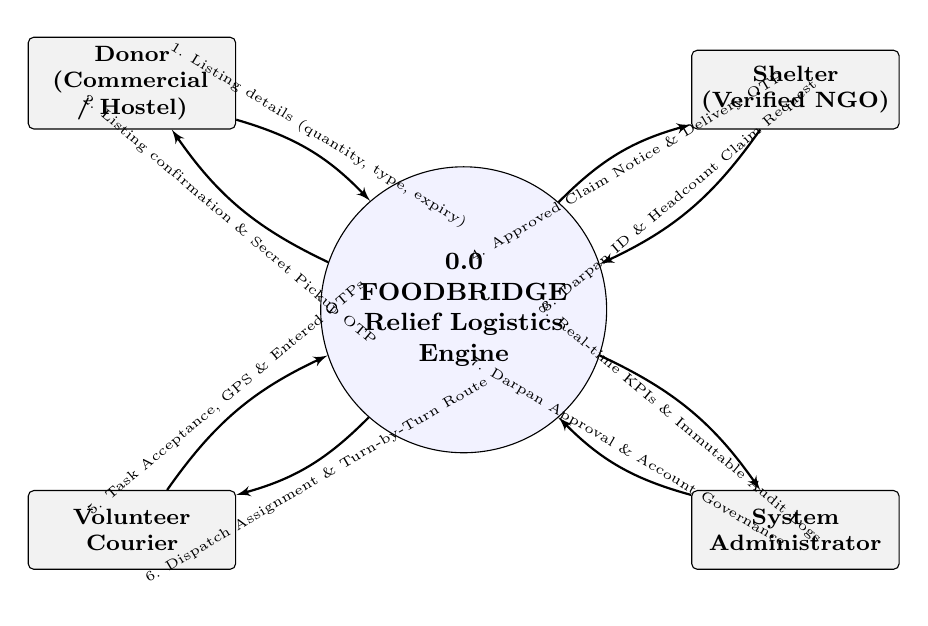
\begin{tikzpicture}[node distance=2.2cm, auto,
    proc/.style={circle, draw=black, fill=blue!5, text width=3.0cm, text centered, font=\small\bfseries, minimum height=3.0cm},
    entity/.style={rectangle, draw=black, fill=gray!10, text width=2.4cm, text centered, rounded corners=2pt, minimum height=1.0cm, font=\footnotesize\bfseries},
    flow/.style={draw, -latex', thick}]

    % Center Process
    \node [proc] (sys) {0.0\\FOODBRIDGE\\Relief Logistics\\Engine};

    % Surrounding Entities
    \node [entity, above left=1.0cm and 1.6cm of sys] (donor) {Donor\\(Commercial / Hostel)};
    \node [entity, above right=1.0cm and 1.6cm of sys] (shelter) {Shelter\\(Verified NGO)};
    \node [entity, below left=1.0cm and 1.6cm of sys] (vol) {Volunteer\\Courier};
    \node [entity, below right=1.0cm and 1.6cm of sys] (admin) {System\\Administrator};

    % Flows with Donor
    \draw [flow] (donor) to [bend left=15] node[above, sloped, font=\tiny] {1. Listing details (quantity, type, expiry)} (sys);
    \draw [flow] (sys) to [bend left=15] node[below, sloped, font=\tiny] {2. Listing confirmation \& Secret Pickup OTP} (donor);

    % Flows with Shelter
    \draw [flow] (shelter) to [bend left=15] node[above, sloped, font=\tiny] {3. Darpan ID \& Headcount Claim Request} (sys);
    \draw [flow] (sys) to [bend left=15] node[below, sloped, font=\tiny] {4. Approved Claim Notice \& Delivery OTP} (shelter);

    % Flows with Volunteer
    \draw [flow] (vol) to [bend left=15] node[above, sloped, font=\tiny] {5. Task Acceptance, GPS \& Entered OTPs} (sys);
    \draw [flow] (sys) to [bend left=15] node[below, sloped, font=\tiny] {6. Dispatch Assignment \& Turn-by-Turn Route} (vol);

    % Flows with Admin
    \draw [flow] (admin) to [bend left=15] node[above, sloped, font=\tiny] {7. Darpan Approval \& Account Governance} (sys);
    \draw [flow] (sys) to [bend left=15] node[below, sloped, font=\tiny] {8. Real-time KPIs \& Immutable Audit Logs} (admin);
\end{tikzpicture}
\caption{DFD Level 0 (Context Diagram)}
\label{fig:dfd_0}
\end{figure}

The Level-1 Data Flow Diagram decomposes the system into six core operational processes and four dedicated data stores: Users and Accreditation Records (D1), Surplus Donations (D2), Distribution Records (D3), and Immutable Audit Trail Logs (D4).

\begin{figure}[H]
\centering
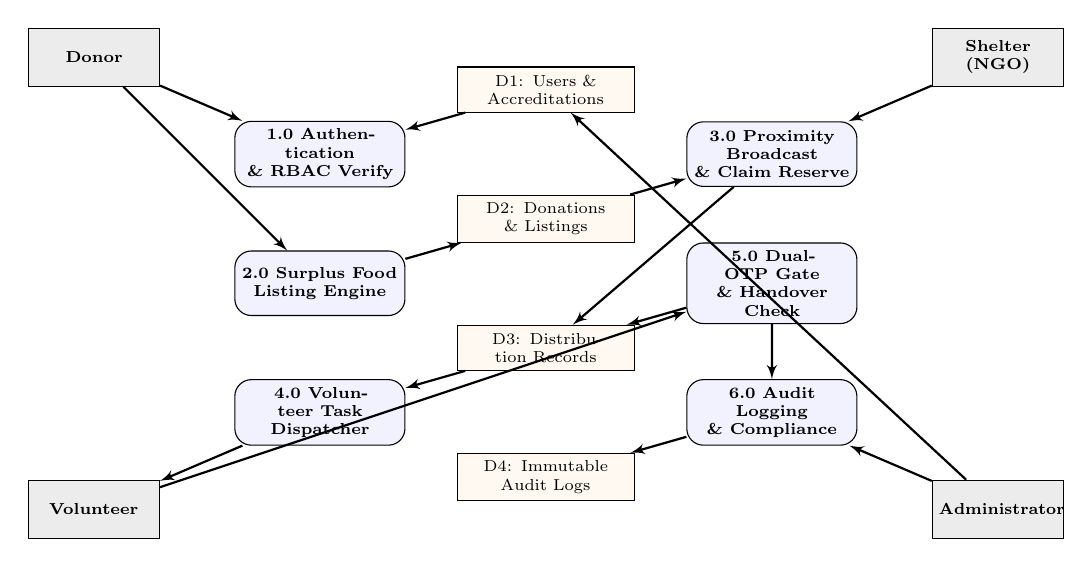
\begin{tikzpicture}[scale=0.82, every node/.style={transform shape},
    proc/.style={rectangle, draw=black, fill=blue!5, text width=2.4cm, text centered, rounded corners=6pt, minimum height=1.0cm, font=\scriptsize\bfseries},
    dstore/.style={rectangle, draw=black, fill=orange!5, text width=2.5cm, text centered, minimum height=0.7cm, font=\scriptsize},
    entity/.style={rectangle, draw=black, fill=gray!15, text width=1.8cm, text centered, minimum height=0.9cm, font=\scriptsize\bfseries},
    flow/.style={draw, -latex', thick}]

    % Entities
    \node [entity] (e_donor) at (0, 7) {Donor};
    \node [entity] (e_shelter) at (14, 7) {Shelter (NGO)};
    \node [entity] (e_vol) at (0, 0) {Volunteer};
    \node [entity] (e_admin) at (14, 0) {Administrator};

    % Processes
    \node [proc] (p1) at (3.5, 5.5) {1.0 Authentication\\\& RBAC Verify};
    \node [proc] (p2) at (3.5, 3.5) {2.0 Surplus Food\\Listing Engine};
    \node [proc] (p3) at (10.5, 5.5) {3.0 Proximity Broadcast\\\& Claim Reserve};
    \node [proc] (p4) at (3.5, 1.5) {4.0 Volunteer Task\\Dispatcher};
    \node [proc] (p5) at (10.5, 3.5) {5.0 Dual-OTP Gate\\\& Handover Check};
    \node [proc] (p6) at (10.5, 1.5) {6.0 Audit Logging\\\& Compliance};

    % Data Stores
    \node [dstore] (d1) at (7, 6.5) {D1: Users \& Accreditations};
    \node [dstore] (d2) at (7, 4.5) {D2: Donations \& Listings};
    \node [dstore] (d3) at (7, 2.5) {D3: Distribution Records};
    \node [dstore] (d4) at (7, 0.5) {D4: Immutable Audit Logs};

    % Connectors
    \draw [flow] (e_donor) -- (p1);
    \draw [flow] (e_donor) -- (p2);
    \draw [flow] (p2) -- (d2);
    \draw [flow] (d2) -- (p3);
    \draw [flow] (e_shelter) -- (p3);
    \draw [flow] (p3) -- (d3);
    \draw [flow] (d3) -- (p4);
    \draw [flow] (p4) -- (e_vol);
    \draw [flow] (e_vol) -- (p5);
    \draw [flow] (p5) -- (d3);
    \draw [flow] (p5) -- (p6);
    \draw [flow] (p6) -- (d4);
    \draw [flow] (e_admin) -- (p6);
    \draw [flow] (e_admin) -- (d1);
    \draw [flow] (d1) -- (p1);
\end{tikzpicture}
\caption{DFD Level 1}
\label{fig:dfd_1}
\end{figure}

\subsection{Use Case Diagram}
The Use Case Diagram defines the interactions between the four system actors and the core functional use cases provided by FoodBridge. The system has four primary actors: Donors list surplus meals and sign the Food Safety Charter; accredited Shelters inspect nearby feeds and reserve claims based on resident headcount; Volunteers accept dispatches and execute physical handovers; and Administrators moderate accreditations and inspect audit trails.

\begin{figure}[H]
\centering
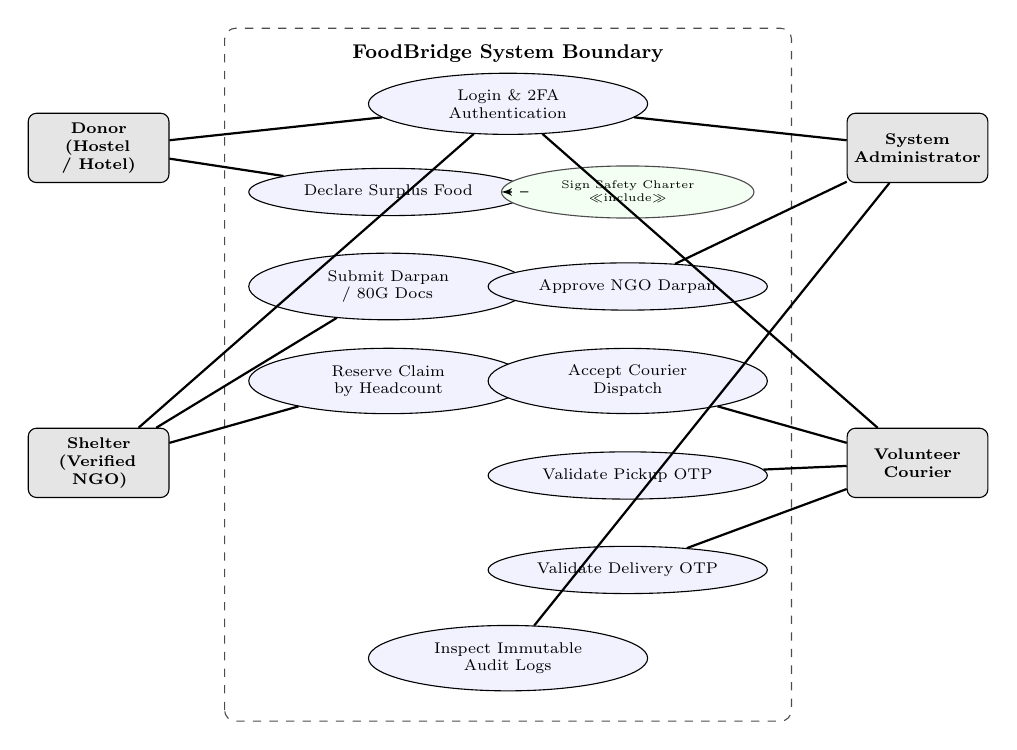
\begin{tikzpicture}[scale=0.80, every node/.style={transform shape},
    actor/.style={rectangle, draw=black, fill=gray!20, text width=2.0cm, text centered, rounded corners=3pt, minimum height=1.1cm, font=\scriptsize\bfseries},
    usecase/.style={ellipse, draw=black, fill=blue!5, text width=2.9cm, text centered, minimum height=0.75cm, font=\scriptsize},
    subcase/.style={ellipse, draw=black!70, fill=green!5, text width=2.6cm, text centered, minimum height=0.70cm, font=\tiny},
    link/.style={draw, thick}]

    % System Box
    \draw [draw=black!70, dashed, rounded corners=4pt] (2.8, -0.6) rectangle (11.8, 10.4);
    \node [font=\bfseries\small] at (7.3, 10.0) {FoodBridge System Boundary};

    % Actors
    \node [actor] (a_donor) at (0.8, 8.5) {Donor\\(Hostel / Hotel)};
    \node [actor] (a_shelter) at (0.8, 3.5) {Shelter\\(Verified NGO)};
    \node [actor] (a_vol) at (13.8, 3.5) {Volunteer\\Courier};
    \node [actor] (a_admin) at (13.8, 8.5) {System\\Administrator};

    % Use cases
    \node [usecase] (uc_login) at (7.3, 9.2) {Login \& 2FA Authentication};
    \node [usecase] (uc_list) at (5.4, 7.8) {Declare Surplus Food};
    \node [subcase] (uc_charter) at (9.2, 7.8) {Sign Safety Charter\\$\ll$include$\gg$};
    \node [usecase] (uc_darpan) at (5.4, 6.3) {Submit Darpan / 80G Docs};
    \node [usecase] (uc_claim) at (5.4, 4.8) {Reserve Claim by Headcount};
    \node [usecase] (uc_accept) at (9.2, 4.8) {Accept Courier Dispatch};
    \node [usecase] (uc_pickup) at (9.2, 3.3) {Validate Pickup OTP};
    \node [usecase] (uc_deliv) at (9.2, 1.8) {Validate Delivery OTP};
    \node [usecase] (uc_admin_app) at (9.2, 6.3) {Approve NGO Darpan};
    \node [usecase] (uc_audit) at (7.3, 0.4) {Inspect Immutable Audit Logs};

    % Actor associations
    \draw [link] (a_donor) -- (uc_login);
    \draw [link] (a_donor) -- (uc_list);
    \draw [draw=black, dashed, -latex'] (uc_list) -- (uc_charter);
    \draw [link] (a_shelter) -- (uc_login);
    \draw [link] (a_shelter) -- (uc_darpan);
    \draw [link] (a_shelter) -- (uc_claim);
    \draw [link] (a_vol) -- (uc_login);
    \draw [link] (a_vol) -- (uc_accept);
    \draw [link] (a_vol) -- (uc_pickup);
    \draw [link] (a_vol) -- (uc_deliv);
    \draw [link] (a_admin) -- (uc_login);
    \draw [link] (a_admin) -- (uc_admin_app);
    \draw [link] (a_admin) -- (uc_audit);
\end{tikzpicture}
\caption{Use Case Diagram}
\label{fig:use_case}
\end{figure}

\subsection{Activity Diagram}
The Activity Diagram details the end-to-end control flow of the food redistribution lifecycle, capturing the safety charter declaration, Darpan check branch, task acceptance, and dual-OTP verification steps.

\begin{figure}[H]
\centering
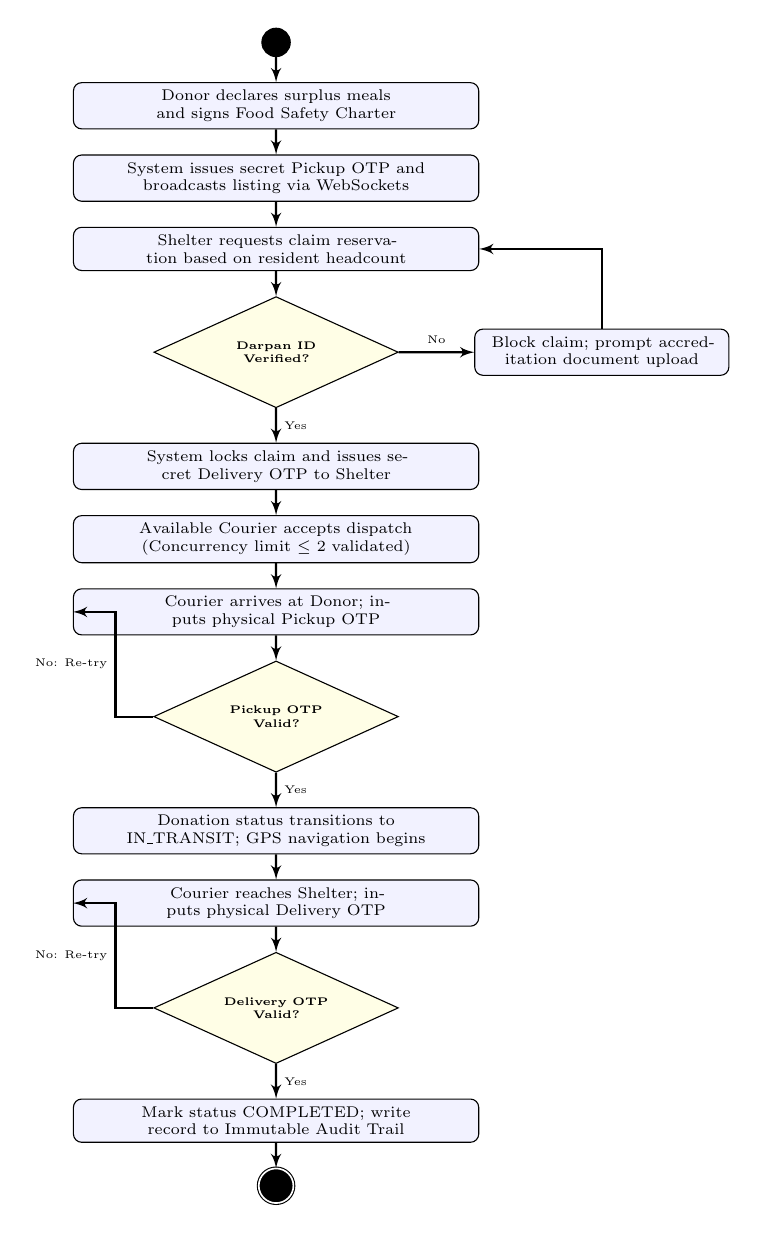
\begin{tikzpicture}[scale=0.80, every node/.style={transform shape},
    startstop/.style={circle, draw=black, fill=black, minimum size=0.45cm},
    endstop/.style={circle, draw=black, double, fill=black, minimum size=0.55cm},
    activity/.style={rectangle, draw=black, fill=blue!5, text width=6.2cm, text centered, rounded corners=3pt, minimum height=0.68cm, font=\scriptsize},
    decision/.style={diamond, draw=black, fill=yellow!10, aspect=2.2, text width=2.4cm, text centered, font=\tiny\bfseries},
    flow/.style={draw, -latex', thick}]

    \node [startstop] (start) at (0, 0) {};
    \node [activity, below=0.40cm of start] (a1) {Donor declares surplus meals and signs Food Safety Charter};
    \node [activity, below=0.40cm of a1] (a2) {System issues secret Pickup OTP and broadcasts listing via WebSockets};
    \node [activity, below=0.40cm of a2] (a3) {Shelter requests claim reservation based on resident headcount};
    \node [decision, below=0.40cm of a3] (d1) {Darpan ID\\Verified?};
    \node [activity, right=1.2cm of d1, text width=3.8cm] (err_darpan) {Block claim; prompt accreditation document upload};
    \node [activity, below=0.55cm of d1] (a4) {System locks claim and issues secret Delivery OTP to Shelter};
    \node [activity, below=0.40cm of a4] (a5) {Available Courier accepts dispatch (Concurrency limit $\le$ 2 validated)};
    \node [activity, below=0.40cm of a5] (a6) {Courier arrives at Donor; inputs physical Pickup OTP};
    \node [decision, below=0.40cm of a6] (d2) {Pickup OTP\\Valid?};
    \node [activity, below=0.55cm of d2] (a7) {Donation status transitions to IN\_TRANSIT; GPS navigation begins};
    \node [activity, below=0.40cm of a7] (a8) {Courier reaches Shelter; inputs physical Delivery OTP};
    \node [decision, below=0.40cm of a8] (d3) {Delivery OTP\\Valid?};
    \node [activity, below=0.55cm of d3] (a9) {Mark status COMPLETED; write record to Immutable Audit Trail};
    \node [endstop, below=0.40cm of a9] (finish) {};

    \draw [flow] (start) -- (a1);
    \draw [flow] (a1) -- (a2);
    \draw [flow] (a2) -- (a3);
    \draw [flow] (a3) -- (d1);
    \draw [flow] (d1) -- node[right, font=\tiny] {Yes} (a4);
    \draw [flow] (d1) -- node[above, font=\tiny] {No} (err_darpan);
    \draw [flow] (err_darpan) |- (a3);
    \draw [flow] (a4) -- (a5);
    \draw [flow] (a5) -- (a6);
    \draw [flow] (a6) -- (d2);
    \draw [flow] (d2) -- node[right, font=\tiny] {Yes} (a7);
    \draw [flow] (d2.west) -- ++(-0.6,0) |- node[near start, left, font=\tiny] {No: Re-try} (a6.west);
    \draw [flow] (a7) -- (a8);
    \draw [flow] (a8) -- (d3);
    \draw [flow] (d3) -- node[right, font=\tiny] {Yes} (a9);
    \draw [flow] (d3.west) -- ++(-0.6,0) |- node[near start, left, font=\tiny] {No: Re-try} (a8.west);
    \draw [flow] (a9) -- (finish);
\end{tikzpicture}
\caption{Activity Diagram for Food Redistribution Lifecycle}
\label{fig:activity_diag}
\end{figure}

\subsection{Class Diagram}
The Class Diagram models the core entity classes, value objects, and business service providers that form the structural foundation of the FoodBridge codebase.

\begin{figure}[H]
\centering
\begin{tikzpicture}[scale=0.74, every node/.style={transform shape},
    classbox/.style={rectangle, draw=black, fill=white, text width=5.6cm, inner sep=4pt, font=\scriptsize},
    rel/.style={draw, thick, -open triangle 60},
    assoc/.style={draw, thick, -latex'}]

    % Class: AppUser
    \node [classbox] (user) at (0, 7.5) {
        \textbf{AppUser}\\[0.05cm]
        \hline
        - id: String (UUID)\\
        - fullName: String\\
        - email: String\\
        - role: UserRole\\
        - phone: String\\
        - darpanId: String\\
        - isVerified: bool\\[0.05cm]
        \hline
        + login(): Future$\langle$bool$\rangle$\\
        + updateProfile(): Future$\langle$void$\rangle$\\
        + verify2FA(code): bool
    };

    % Class: Donation
    \node [classbox] (donation) at (8.5, 7.5) {
        \textbf{Donation}\\[0.05cm]
        \hline
        - id: String (UUID)\\
        - donorId: String\\
        - title: String\\
        - foodType: FoodType\\
        - quantityKg: double\\
        - expiryTime: DateTime\\
        - pickupOTP: String\\
        - status: DonationStatus\\[0.05cm]
        \hline
        + createListing(): Future$\langle$void$\rangle$\\
        + cancelListing(): Future$\langle$void$\rangle$\\
        + markInTransit(): void
    };

    % Class: DistributionRecord
    \node [classbox] (dist) at (8.5, 1.8) {
        \textbf{DistributionRecord}\\[0.05cm]
        \hline
        - id: String (UUID)\\
        - donationId: String\\
        - shelterId: String\\
        - volunteerId: String\\
        - beneficiaryCount: int\\
        - deliveryOTP: String\\
        - pickupTime: DateTime\\
        - deliveryTime: DateTime\\[0.05cm]
        \hline
        + reserveClaim(): bool\\
        + verifyPickup(otp): bool\\
        + verifyDelivery(otp): bool
    };

    % Class: AuditLogEntry
    \node [classbox] (audit) at (0, 1.8) {
        \textbf{AuditLogEntry}\\[0.05cm]
        \hline
        - logId: String (UUID)\\
        - actorId: String\\
        - action: String\\
        - targetResource: String\\
        - timestamp: DateTime\\
        - ipAddress: String\\[0.05cm]
        \hline
        + appendImmutableLog(): void\\
        + verifyIntegrityHash(): bool
    };

    \draw [assoc] (user) -- node[above, font=\tiny] {1 \quad creates \quad 0..*} (donation);
    \draw [assoc] (donation) -- node[right, font=\tiny] {1 \quad fulfilled\_by \quad 1} (dist);
    \draw [assoc] (user) -- node[above, font=\tiny, sloped] {1 \quad claims/delivers \quad 0..*} (dist);
    \draw [assoc] (user) -- node[left, font=\tiny] {1 \quad generates \quad 0..*} (audit);
\end{tikzpicture}
\caption{Class Diagram}
\label{fig:class_diagram}
\end{figure}

\subsection{Sequence Diagram}
The Sequence Diagram illustrates the chronological message exchange between five lifelines during a complete surplus food redistribution transaction.

\begin{figure}[H]
\centering
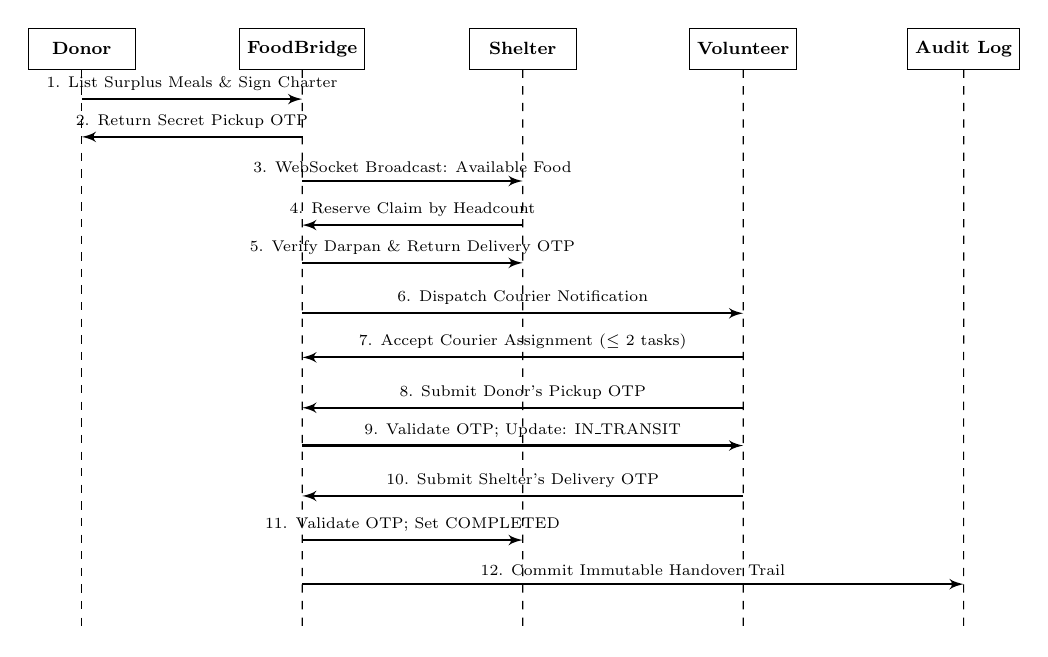
\begin{tikzpicture}[scale=0.80, every node/.style={transform shape}]
    % Lifelines
    \node (d) at (0,0) [draw, fill=white, minimum width=1.7cm, minimum height=0.65cm, font=\bfseries\footnotesize] {Donor};
    \node (s) at (3.5,0) [draw, fill=white, minimum width=1.7cm, minimum height=0.65cm, font=\bfseries\footnotesize] {FoodBridge};
    \node (sh) at (7.0,0) [draw, fill=white, minimum width=1.7cm, minimum height=0.65cm, font=\bfseries\footnotesize] {Shelter};
    \node (v) at (10.5,0) [draw, fill=white, minimum width=1.7cm, minimum height=0.65cm, font=\bfseries\footnotesize] {Volunteer};
    \node (a) at (14.0,0) [draw, fill=white, minimum width=1.7cm, minimum height=0.65cm, font=\bfseries\footnotesize] {Audit Log};

    \draw [dashed] (d) -- (0,-9.2);
    \draw [dashed] (s) -- (3.5,-9.2);
    \draw [dashed] (sh) -- (7.0,-9.2);
    \draw [dashed] (v) -- (10.5,-9.2);
    \draw [dashed] (a) -- (14.0,-9.2);

    % Sequence Messages
    \draw [-latex', thick] (d) ++(0,-0.8) -- node[above, font=\scriptsize] {1. List Surplus Meals \& Sign Charter} (3.5,-0.8);
    \draw [-latex', thick] (3.5,-1.4) -- node[above, font=\scriptsize] {2. Return Secret Pickup OTP} (0,-1.4);
    \draw [-latex', thick] (3.5,-2.1) -- node[above, font=\scriptsize] {3. WebSocket Broadcast: Available Food} (7.0,-2.1);
    \draw [-latex', thick] (sh) ++(0,-2.8) -- node[above, font=\scriptsize] {4. Reserve Claim by Headcount} (3.5,-2.8);
    \draw [-latex', thick] (3.5,-3.4) -- node[above, font=\scriptsize] {5. Verify Darpan \& Return Delivery OTP} (7.0,-3.4);
    \draw [-latex', thick] (3.5,-4.2) -- node[above, font=\scriptsize] {6. Dispatch Courier Notification} (10.5,-4.2);
    \draw [-latex', thick] (v) ++(0,-4.9) -- node[above, font=\scriptsize] {7. Accept Courier Assignment ($\le$ 2 tasks)} (3.5,-4.9);
    \draw [-latex', thick] (v) ++(0,-5.7) -- node[above, font=\scriptsize] {8. Submit Donor's Pickup OTP} (3.5,-5.7);
    \draw [-latex', thick] (3.5,-6.3) -- node[above, font=\scriptsize] {9. Validate OTP; Update: IN\_TRANSIT} (10.5,-6.3);
    \draw [-latex', thick] (v) ++(0,-7.1) -- node[above, font=\scriptsize] {10. Submit Shelter's Delivery OTP} (3.5,-7.1);
    \draw [-latex', thick] (3.5,-7.8) -- node[above, font=\scriptsize] {11. Validate OTP; Set COMPLETED} (7.0,-7.8);
    \draw [-latex', thick] (3.5,-8.5) -- node[above, font=\scriptsize] {12. Commit Immutable Handover Trail} (14.0,-8.5);
\end{tikzpicture}
\caption{Sequence Diagram for Listing, Claim and Dual-OTP Handover}
\label{fig:seq_diagram}
\end{figure}

\subsection{Collaboration Diagram}
The Collaboration Diagram displays the structural relationships and numbered message sequences connecting the collaborating runtime objects.

\begin{figure}[H]
\centering
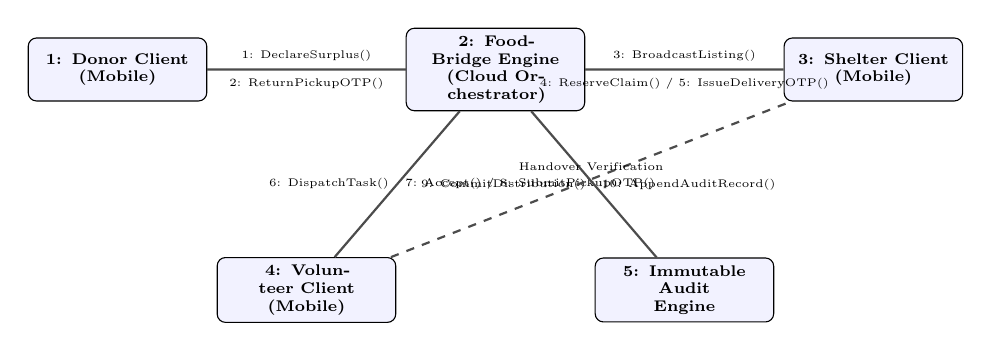
\begin{tikzpicture}[scale=0.80, every node/.style={transform shape},
    obj/.style={rectangle, draw=black, fill=blue!5, text width=2.6cm, text centered, rounded corners=3pt, minimum height=1.0cm, font=\scriptsize\bfseries},
    conn/.style={draw=black!70, thick}]

    % Objects
    \node [obj] (donor) at (0, 4) {1: Donor Client\\(Mobile)};
    \node [obj] (server) at (6, 4) {2: FoodBridge Engine\\(Cloud Orchestrator)};
    \node [obj] (shelter) at (12, 4) {3: Shelter Client\\(Mobile)};
    \node [obj] (vol) at (3, 0.5) {4: Volunteer Client\\(Mobile)};
    \node [obj] (audit) at (9, 0.5) {5: Immutable Audit\\Engine};

    % Connections and message annotations
    \draw [conn] (donor) -- node[above, font=\tiny] {1: DeclareSurplus()} node[below, font=\tiny] {2: ReturnPickupOTP()} (server);
    \draw [conn] (server) -- node[above, font=\tiny] {3: BroadcastListing()} node[below, font=\tiny] {4: ReserveClaim() / 5: IssueDeliveryOTP()} (shelter);
    \draw [conn] (server) -- node[left, font=\tiny] {6: DispatchTask()} node[right, font=\tiny] {7: Accept() / 8: SubmitPickupOTP()} (vol);
    \draw [conn] (server) -- node[left, font=\tiny] {9: CommitDistribution()} node[right, font=\tiny] {10: AppendAuditRecord()} (audit);
    \draw [conn, dashed] (vol) -- node[above, font=\tiny] {Handover Verification} (shelter);
\end{tikzpicture}
\caption{Collaboration Diagram}
\label{fig:collab_diagram}
\end{figure}

\subsection{Database Diagrams}
\subsubsection{Entity Relationship (ER) Diagram}
The database schema comprises four primary entities and one audit log entity. One registered donor lists multiple surplus donations. Each donation corresponds to a single completed distribution record. Accredited shelters reserve claims, while couriers execute deliveries.

\begin{figure}[H]
\centering
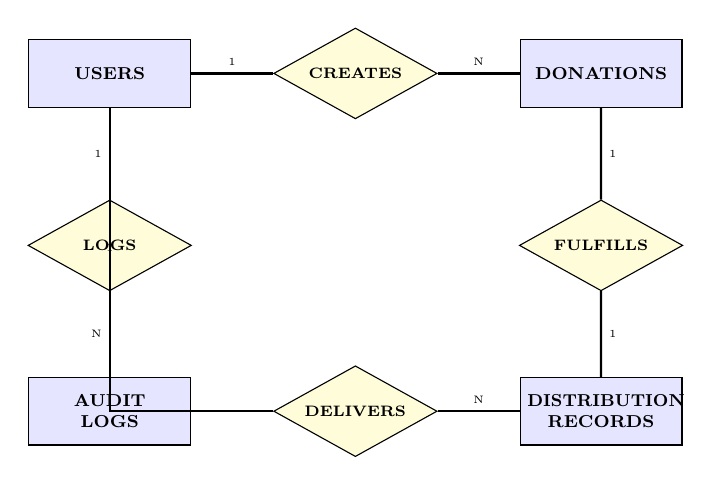
\begin{tikzpicture}[scale=0.78, every node/.style={transform shape},
    entity/.style={rectangle, draw=black, fill=blue!10, text width=2.4cm, text centered, minimum height=1.1cm, font=\footnotesize\bfseries},
    relation/.style={diamond, draw=black, fill=yellow!15, aspect=1.8, text width=1.7cm, text centered, font=\scriptsize\bfseries},
    attr/.style={ellipse, draw=black!70, fill=white, text width=1.8cm, text centered, font=\tiny},
    link/.style={draw, thick}]

    % Entities
    \node [entity] (e_user) at (1.5, 6) {USERS};
    \node [entity] (e_donation) at (9.5, 6) {DONATIONS};
    \node [entity] (e_dist) at (9.5, 0.5) {DISTRIBUTION\\RECORDS};
    \node [entity] (e_audit) at (1.5, 0.5) {AUDIT\\LOGS};

    % Relationships
    \node [relation] (r_creates) at (5.5, 6) {CREATES};
    \node [relation] (r_fulfills) at (9.5, 3.2) {FULFILLS};
    \node [relation] (r_logs) at (1.5, 3.2) {LOGS};
    \node [relation] (r_delivers) at (5.5, 0.5) {DELIVERS};

    % Connections
    \draw [link] (e_user) -- node[above, font=\tiny] {1} (r_creates);
    \draw [link] (r_creates) -- node[above, font=\tiny] {N} (e_donation);
    \draw [link] (e_donation) -- node[right, font=\tiny] {1} (r_fulfills);
    \draw [link] (r_fulfills) -- node[right, font=\tiny] {1} (e_dist);
    \draw [link] (e_user) -- node[left, font=\tiny] {1} (r_logs);
    \draw [link] (r_logs) -- node[left, font=\tiny] {N} (e_audit);
    \draw [link] (e_user) |- node[near start, above, font=\tiny] {1} (r_delivers);
    \draw [link] (r_delivers) -- node[above, font=\tiny] {N} (e_dist);
\end{tikzpicture}
\caption{Entity Relationship Diagram}
\label{fig:er_diagram}
\end{figure}

\subsubsection{Table Relationships}
The detailed relational design, primary keys, foreign key references, and constraints are documented in Table 5.1.

\begin{table}[H]
\centering
\caption{Database Tables and Relationships}
\label{tab:db_tables}
\resizebox{\textwidth}{!}{
\begin{tabular}{|l|p{7.5cm}|p{5.5cm}|}
    \hline
    \textbf{Table} & \textbf{Key Fields} & \textbf{Relationship / Description} \\
    \hline
    \textbf{users} & id (PK, UUID), email (unique), full\_name, role, phone, darpan\_id, is\_verified, created\_at & Master registry. One user $\rightarrow$ many donations, claims, or courier deliveries. \\
    \hline
    \textbf{donations} & id (PK, UUID), donor\_id (FK $\rightarrow$ users.id), title, food\_type, quantity\_kg, expiry\_time, pickup\_otp, status, created\_at & Many donations $\rightarrow$ one donor. Fulfilled by exactly one distribution record. \\
    \hline
    \textbf{distribution\_records} & id (PK, UUID), donation\_id (FK $\rightarrow$ donations.id), shelter\_id (FK $\rightarrow$ users.id), volunteer\_id (FK $\rightarrow$ users.id), beneficiary\_count, delivery\_otp, status, completed\_at & Connects claimed donation, receiving charitable shelter, and delivering courier. \\
    \hline
    \textbf{audit\_logs} & id (PK, UUID), actor\_id (FK $\rightarrow$ users.id), action, resource, details, ip\_address, timestamp & Immutable system audit trail. Every privileged action is linked to an authenticated actor. \\
    \hline
    \textbf{otp\_codes} & id (PK, UUID), user\_id (FK $\rightarrow$ users.id), code, purpose, expires\_at, is\_consumed & Ephemeral token records validating 2FA login and emergency resets. \\
    \hline
\end{tabular}
}
\end{table}

% ==============================================================================
% CHAPTER 6: IMPLEMENTATION
% ==============================================================================
\newpage
\section{IMPLEMENTATION}

\subsection{Technology}
The complete technology stack utilized for the development and testing of FoodBridge is summarized in Table 6.1.

\begin{table}[H]
\centering
\caption{Technology Stack}
\label{tab:tech_stack}
\begin{tabularx}{\textwidth}{|l|l|X|}
    \hline
    \textbf{Layer} & \textbf{Technology} & \textbf{Reason for Choice} \\
    \hline
    Mobile Client & Flutter 3.24+ (Dart 3.5+) & Unified single-codebase development for Android, iOS and Web with 120 FPS native performance. \\
    \hline
    State Management & Provider \& ChangeNotifier & Predictable state mutations, local optimistic rendering, and testability. \\
    \hline
    Backend / BaaS & Supabase (PostgreSQL 15+) & Real-time WebSockets, integrated Auth engine, and relational SQL integrity. \\
    \hline
    Security Engine & Row Level Security (RLS) & Fine-grained row-level authorization enforced directly at database engine level. \\
    \hline
    Verification Gate & Cryptographic Dual-OTP & Double-blind pickup and delivery token validation preventing falsified deliveries. \\
    \hline
    Offline Storage & SharedPreferences (AES-256) & Resilient local caching preserving active tasks during cellular network dropouts. \\
    \hline
\end{tabularx}
\end{table}

\noindent
\textbf{Implementation completed so far:}
The core architectural layers and stakeholder modules have been implemented and validated end-to-end. These include: (1) Role-Based Access Control and 2FA authentication; (2) The Donor surplus listing interface with dietary classification and Food Safety Charter sign-off; (3) The Shelter (NGO) portal with Darpan accreditation upload and capacity reservation; (4) The Volunteer Courier dispatch console with 2-task throttling and dual-OTP entry; (5) The Admin monitoring dashboard featuring real-time KPI metrics, user moderation, and audit log inspection; and (6) The real-time synchronization engine delivering sub-100ms state broadcasts across distributed clients.

\begin{figure}[H]
\centering
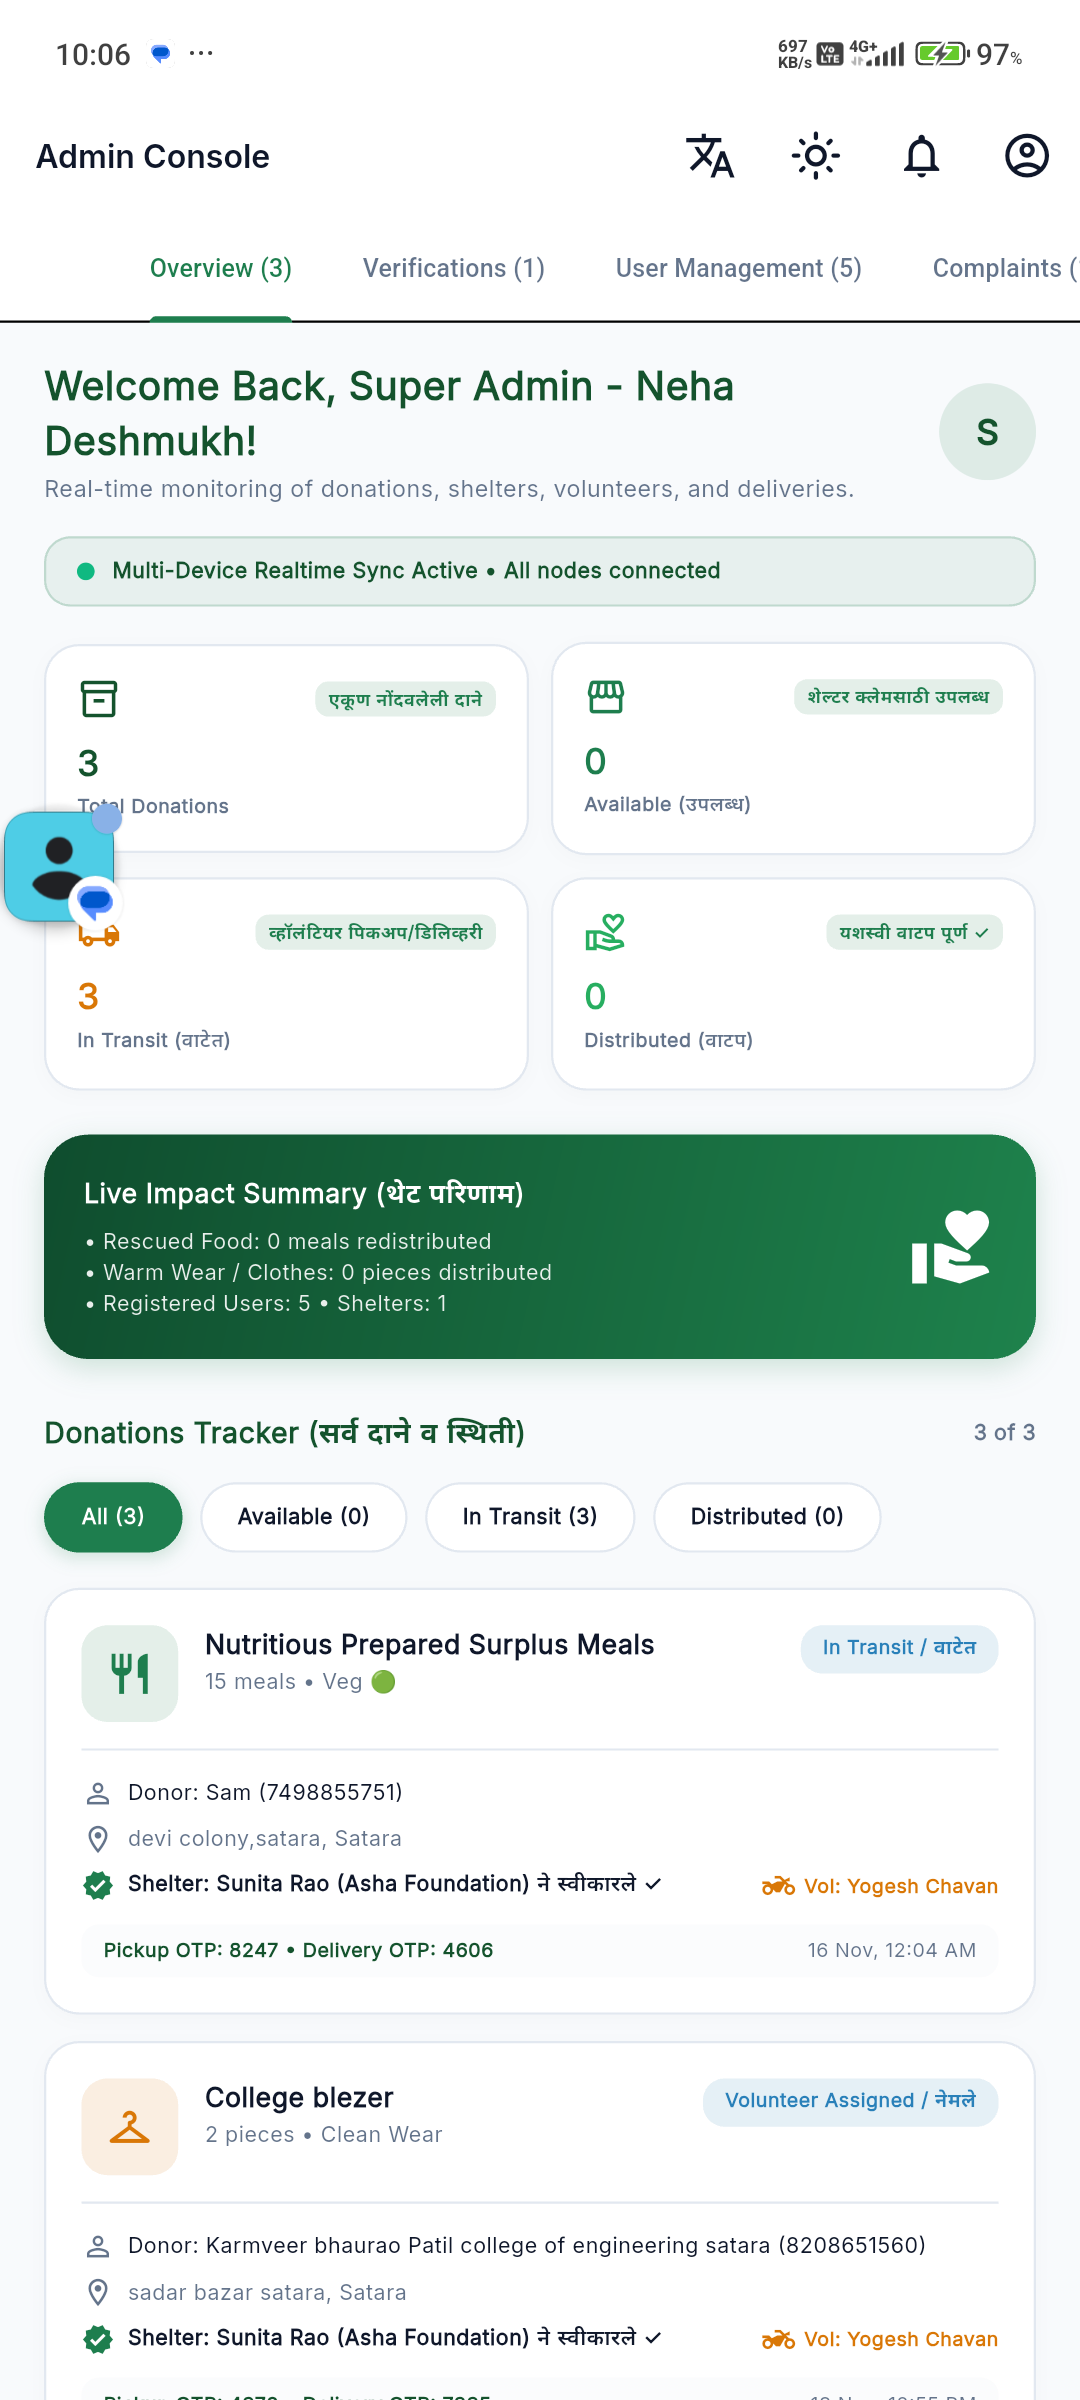
\includegraphics[width=0.82\textwidth]{figures/admin_console.png}
\caption{Admin Console – Real-Time Redistribution Overview (FoodBridge System Overview)}
\label{fig:screen_admin}
\end{figure}

\begin{figure}[H]
\centering
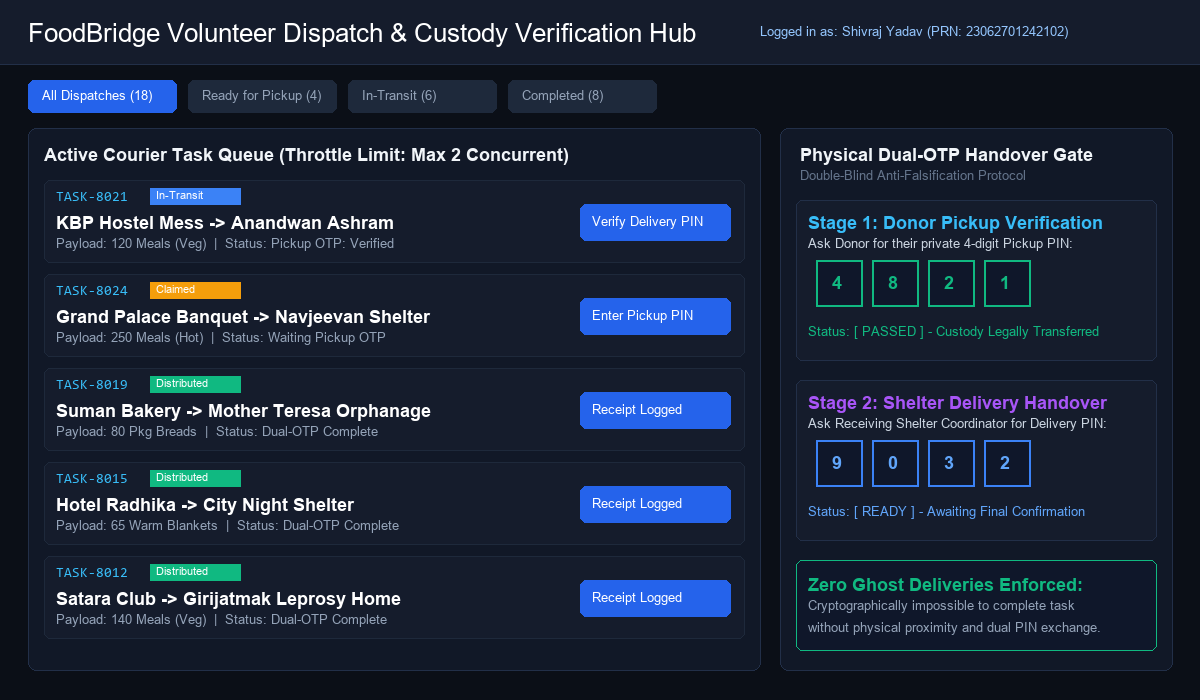
\includegraphics[width=0.82\textwidth]{figures/volunteer_dashboard.png}
\caption{Volunteer Dispatch \& Verification Screen}
\label{fig:screen_volunteer}
\end{figure}

\begin{figure}[H]
\centering
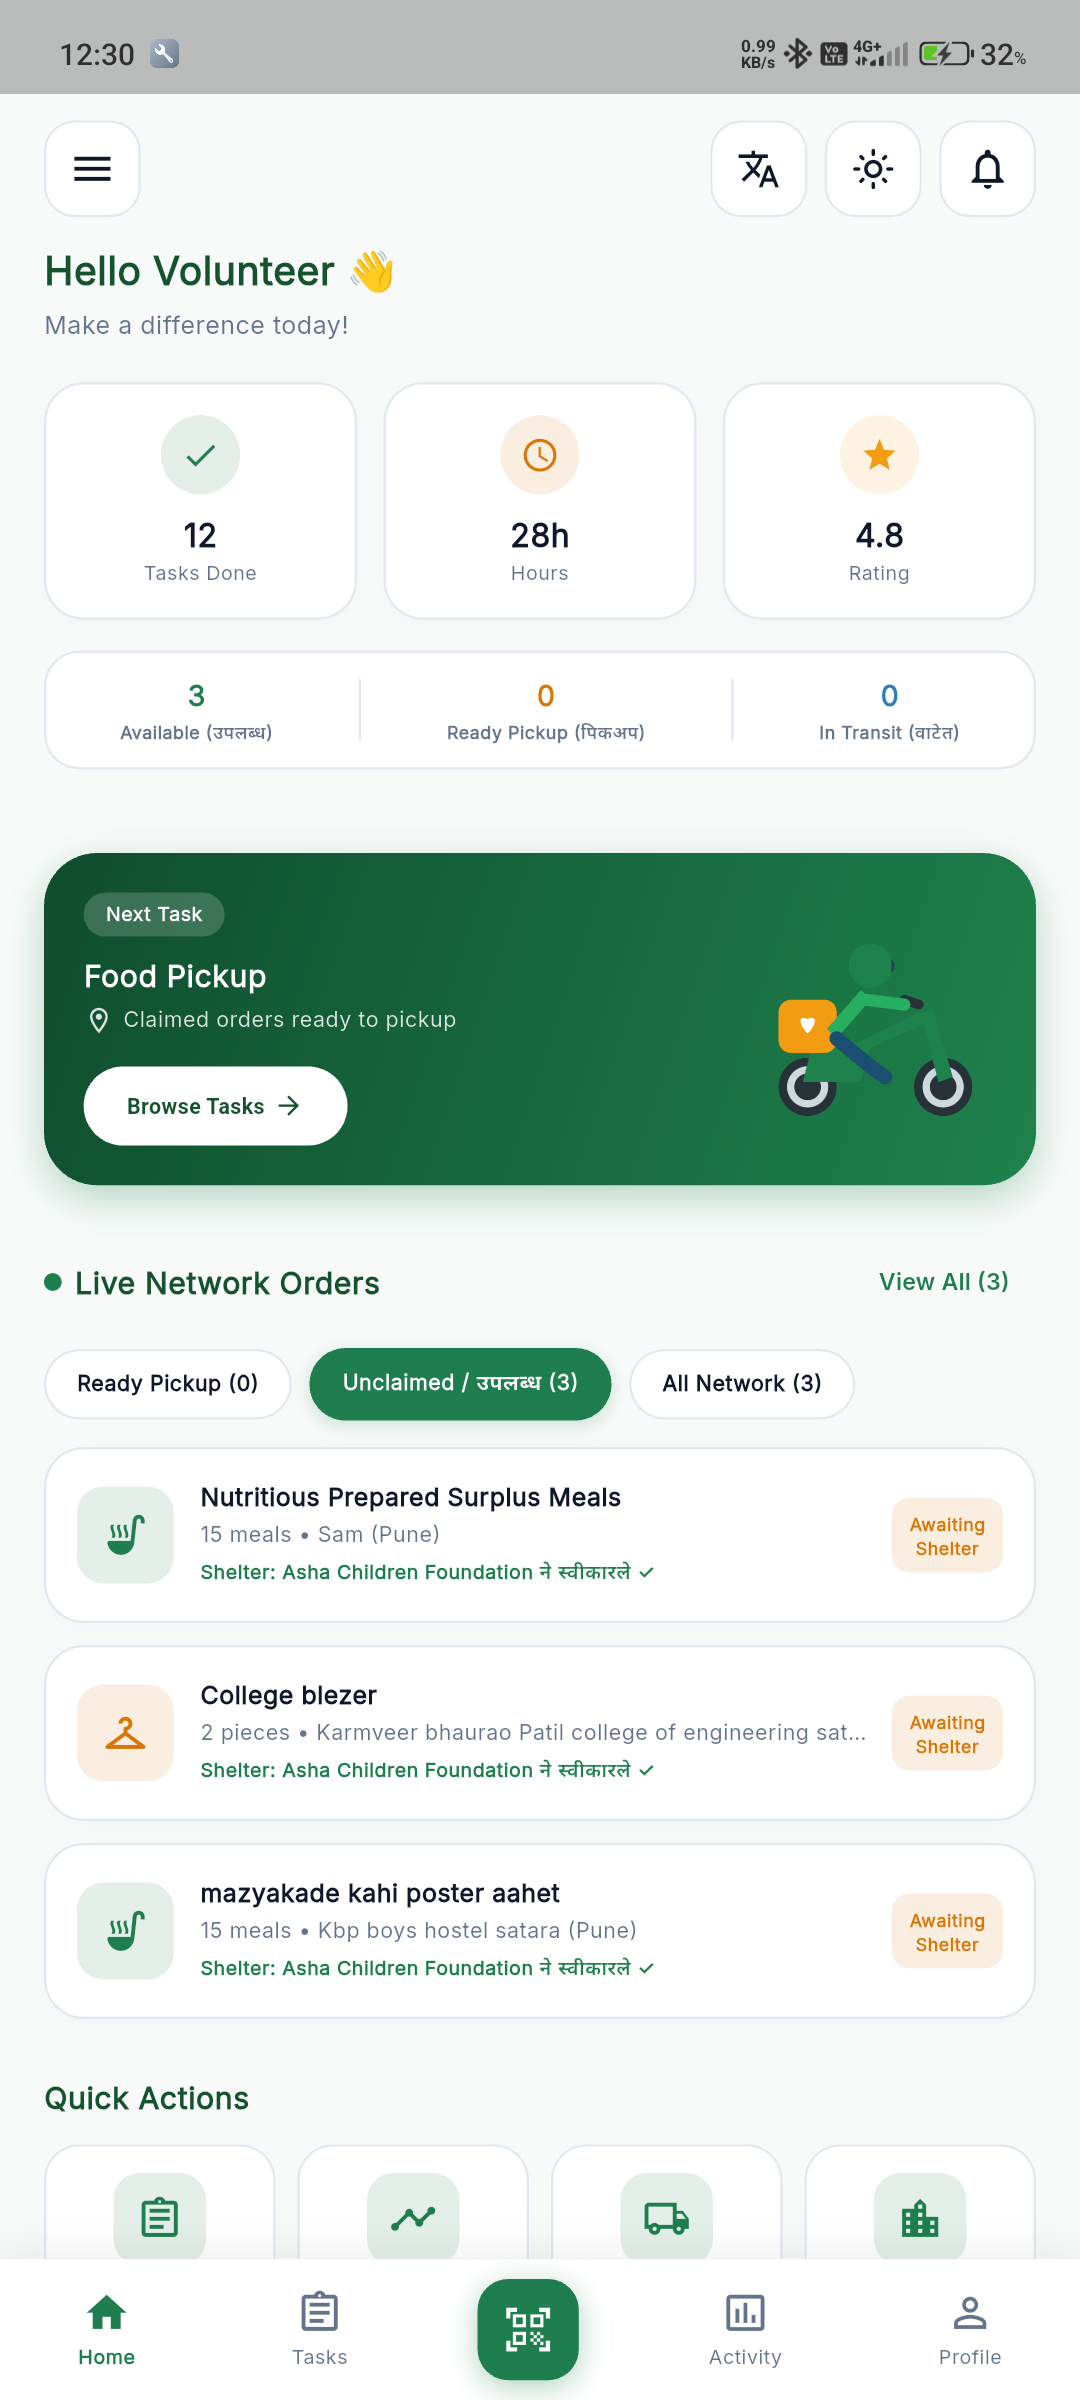
\includegraphics[width=0.82\textwidth]{figures/donation_detail.png}
\caption{Live Donation Details \& API / Transaction Log}
\label{fig:screen_donation}
\end{figure}

\subsection{Steps to be Taken Towards Project Completion}
The sequential roadmap planned to advance FoodBridge from Phase-I design into production-grade urban deployment comprises the following milestones:

\begin{enumerate}
    \item Finalize the problem statement, stakeholder scope, and academic objectives.
    \item Complete comprehensive literature review and regulatory requirement gathering (FSSAI guidelines).
    \item Finalize system architecture, UML models, and Supabase relational schema design.
    \item Implement Role-Based Access Control (RBAC) and JWT authentication with 2FA OTP verification.
    \item Implement Donor Module with dietary tagging (Veg/Non-Veg) and mandatory Food Safety Charter.
    \item Implement Shelter (NGO) Module with Darpan ID and 80G tax accreditation approval workflow.
    \item Build Volunteer Courier dispatch system enforcing concurrent 2-task throttling.
    \item Enforce double-blind cryptographic Dual-OTP handover protocol (Pickup OTP and Delivery OTP).
    \item Deploy real-time WebSocket state distribution ensuring sub-100ms multi-device synchronization.
    \item Implement encrypted local offline caching (SharedPreferences) with optimistic reconciliation.
    \item Conduct extensive unit testing (145+ automated test suites) and physical Android hardware testing.
    \item Final technical documentation, university viva demonstration, and Phase-II deployment launch.
\end{enumerate}

\subsection{Project Scheduling}
\subsubsection{Plan of Action}
The timeline and progress status for Phase-I and Phase-II development activities are outlined in Table 6.2.

\begin{table}[H]
\centering
\caption{Plan of Action}
\label{tab:plan_of_action}
\begin{tabularx}{\textwidth}{|c|X|c|c|}
    \hline
    \textbf{Sr. No.} & \textbf{Activity} & \textbf{Duration} & \textbf{Status} \\
    \hline
    1 & Topic selection, problem definition and literature survey & Jul – Aug 2026 & Completed \\
    \hline
    2 & Requirement analysis and system design (UML, database) & Aug – Sep 2026 & Completed \\
    \hline
    3 & Backend API, Supabase authentication and schema creation & Sep 2026 & Completed \\
    \hline
    4 & Real-time WebSocket sync, Dual-OTP engine and Darpan verifier & Sep – Oct 2026 & Completed \\
    \hline
    5 & Flutter cross-platform mobile client and stakeholder screens & Sep – Oct 2026 & Completed \\
    \hline
    6 & Project Review-II (Hardware deployment \& live testing) & Oct – Nov 2026 & In Progress \\
    \hline
    7 & Municipal pilot deployment and multi-shelter field trial & Dec 2026 – Feb 2027 & Planned \\
    \hline
    8 & Final documentation, project report and University viva & Mar – Apr 2027 & Planned \\
    \hline
\end{tabularx}
\end{table}

\subsection{Cost Estimation}
The software development stack is built upon open-source frameworks (Flutter, Dart, Git) and free-tier cloud infrastructure (Supabase Community Tier). The estimated budget is summarized in Table 6.3.

\begin{table}[H]
\centering
\caption{Approximate Cost Estimation}
\label{tab:cost_est}
\begin{tabularx}{\textwidth}{|l|X|r|}
    \hline
    \textbf{Item} & \textbf{Details} & \textbf{Approx. Cost (\rupee)} \\
    \hline
    Domain Name \& SSL & Production web endpoint with Let's Encrypt SSL (1 year) & 800 – 1,000 \\
    \hline
    SMS Gateway for OTP & Transactional SMS service for live phone OTP handovers & 500 – 1,000 \\
    \hline
    Field Testing \& Logistics & Local transport for hostel/banquet food pickup validation & 1,000 – 1,500 \\
    \hline
    Report Binding \& Printing & University project documentation, hardbound copies & 1,200 – 1,500 \\
    \hline
    \multicolumn{2}{|l|}{\textbf{Total (Approximate)}} & \textbf{3,500 – 5,000} \\
    \hline
\end{tabularx}
\end{table}

\subsection{Team Structure}
The project team comprises four final-year B.Tech students from the Department of Computer Science and Engineering, Karmaveer Bhaurao Patil College of Engineering, Satara. The division of technical responsibilities is defined in Table 6.4.

\begin{table}[H]
\centering
\caption{Team Structure and Work Distribution}
\label{tab:team_dist}
\begin{tabularx}{\textwidth}{|p{0.38\textwidth}|X|}
    \hline
    \textbf{Member} & \textbf{Responsibility} \\
    \hline
    \textbf{1) Yogesh Gurunath Chavan} \newline \footnotesize (PRN: 24062701242502) & Admin Module -- Admin console, user and role management, real-time WebSocket sync engine, dynamic profile resolution, and hardware deployment. \\
    \hline
    \textbf{2) Samruddhi Pramod Sawant} \newline \footnotesize (PRN: 23062701242039) & Donor Module -- Surplus food and wearable clothes declaration, dietary classification (Veg/Non-Veg), Food Safety Charter, and image upload. \\
    \hline
    \textbf{3) Omkar Nilesh Shinde} \newline \footnotesize (PRN: 23062701242121) & Shelter (NGO) Module -- NGO Darpan accreditation verification, 80G tax certificate audit, capacity-based claim allocation, and headcount tracking. \\
    \hline
    \textbf{4) Shivraj Rajendra Yadav} \newline \footnotesize (PRN: 23062701242102) & Volunteer Courier Module -- Courier task dispatch, double-blind Dual-OTP handover protocol, courier concurrency throttling, and integration testing. \\
    \hline
\end{tabularx}
\end{table}

% ==============================================================================
% CHAPTER 7: ADVANTAGES & LIMITATIONS
% ==============================================================================
\newpage
\section{ADVANTAGES \& LIMITATIONS}

\subsection{Advantages}
\begin{enumerate}
    \item \textbf{Enhanced Multi-Layer Security:} Combines Role-Based Access Control (RBAC), 2FA, Supabase Row Level Security, and cryptographic Dual-OTP verification to protect the redistribution chain.
    \item \textbf{Near-Zero Latency Coordination:} Replaces slow, manual phone communication with instantaneous sub-100ms WebSocket broadcasts, preventing perishable food spoilage.
    \item \textbf{Guaranteed Proof of Delivery:} The double-blind PIN protocol (Pickup OTP with Donor, Delivery OTP with Shelter) prevents unauthorized diversion and falsified deliveries.
    \item \textbf{Government Accreditation Integrity:} Ensures that only verified charitable foundations with valid NGO Darpan and 80G registrations can claim surplus food relief.
    \item \textbf{Fair Volunteer Task Distribution:} Restricts volunteers to a maximum of two active tasks concurrently, preventing courier hoarding and delivery delays.
    \item \textbf{Immutable Institutional Accountability:} Permanently archives every donation, reservation, and status mutation in an append-only audit trail for compliance inspection.
    \item \textbf{Cost-Effective and Open-Source:} Built entirely upon modern open-source technologies (Flutter, Dart, Supabase), minimizing financial barriers for charitable deployment.
\end{enumerate}

\subsection{Limitations}
\begin{enumerate}
    \item \textbf{Internet Dependency:} Real-time WebSocket broadcasting and remote database updates require active cellular or Wi-Fi data connectivity.
    \item \textbf{Volunteer Availability in Rural Belts:} In semi-urban or remote rural locations, the speed of redistribution depends on the number of active registered delivery volunteers.
    \item \textbf{Physical Food Quality Verification:} While donors sign a legal Food Safety Charter, verifying microbiological safety currently relies on donor compliance and sensory inspection at pickup.
\end{enumerate}

% ==============================================================================
% CHAPTER 8: APPLICATIONS
% ==============================================================================
\newpage
\section{APPLICATIONS}

\begin{itemize}
    \item \textbf{University and College Campus Dining:} Automated redistribution of surplus meals from university mess halls and student hostels to nearby night shelters.
    \item \textbf{Commercial Hospitality \& Catering:} Transparent salvage of surplus banquet, wedding, and convention food within hours of event conclusion.
    \item \textbf{Charitable Shelter Logistics:} Streamlined intake management for orphanages, elderly care homes, and community kitchens based on real-time resident headcount.
    \item \textbf{Disaster Relief \& Emergency Aid:} Rapid deployment during flood or drought emergencies to route packaged rations and drinking water to displaced citizens.
    \item \textbf{Seasonal Warm Wear Redistribution:} Salvage and distribution of clean winter wear, blankets, and school uniforms alongside food relief pipelines.
\end{itemize}

% ==============================================================================
% CHAPTER 9: FUTURE SCOPE
% ==============================================================================
\newpage
\section{FUTURE SCOPE}

\begin{enumerate}
    \item \textbf{AI-Driven Surplus Volume Forecasting:} Implementing predictive machine learning models to forecast hostel and restaurant surplus quantities based on day-of-week and seasonal consumption patterns.
    \item \textbf{IoT Smart Temperature Boxes:} Integrating temperature-sensor-equipped delivery boxes transmitting telemetry over Bluetooth/LoRaWAN to verify hot/cold chain compliance during transit.
    \item \textbf{Automated Multi-Stop Route Optimization:} Integrating genetic algorithms or Clarke-Wright heuristic routing to dynamically compute optimal multi-stop courier routes.
    \item \textbf{Automated Darpan Web Scraping:} Establishing direct API verification pipelines with the NITI Aayog NGO Darpan portal for instant accreditation approval.
    \item \textbf{Multilingual Voice Interface:} Providing voice prompts in regional Indian languages (Marathi, Hindi) to assist non-literate volunteers and shelter coordinators.
\end{enumerate}

% ==============================================================================
% CHAPTER 10: CONCLUSION
% ==============================================================================
\newpage
\section{CONCLUSION}

\textbf{FOODBRIDGE : Real-Time Surplus Food Redistribution and Logistics Engine} establishes an automated, auditable, and secure bridge between surplus food generators and charitable shelters. By replacing slow, uncoordinated telephone chains with reactive Flutter mobile clients, real-time Supabase WebSocket synchronization, and a double-blind cryptographic Dual-OTP handover gate, FoodBridge addresses the root causes of urban food waste and delivery falsification.

The system enforces strict administrative governance through mandatory NGO Darpan accreditation checks, courier concurrency throttling, and an immutable audit trail. The architectural design, UML models, database schemas, and functional screens developed during Phase-I demonstrate the feasibility, security, and scalability of the platform.

Phase-II will focus on executing physical municipal field trials, conducting multi-shelter capacity tests, and deploying intelligent routing heuristics to maximize meal salvage and eradicate urban hunger across Maharashtra.

% ==============================================================================
% REFERENCES
% ==============================================================================
\newpage
\section*{REFERENCES}
\addcontentsline{toc}{section}{References}

\begin{enumerate}
    \item[{[1]}] United Nations Environment Programme (UNEP), \textit{Food Waste Index Report 2024: Think Eat Save - Tracking Global Food Waste}, Nairobi: UNEP Publications, 2024.
    \item[{[2]}] Food and Agriculture Organization (FAO), \textit{The State of Food Security and Nutrition in the World 2023}, Rome: FAO, 2023.
    \item[{[3]}] C. Shewale et al., ``Multi Factor Authentication and IP Address Restriction based Question Paper Delivery System for Indian Universities,'' \textit{International Journal on Recent and Innovation Trends in Computing and Communication}, vol. 11, no. 10, pp. 390--396, 2023.
    \item[{[4]}] R. Patil, S. Deshmukh, and A. Kulkarni, ``Real-Time Volunteer Routing and Optimization in Urban Relief Distribution Networks,'' in \textit{Proceedings of the IEEE International Conference on Smart Computing and Logistics}, 2023, pp. 112--119.
    \item[{[5]}] S. Kamble and R. Kamble, ``Blockchain-based Competitive Examination System in India,'' \textit{International Journal of Advanced Computer Science}, vol. 14, no. 3, pp. 45--52, 2024.
    \item[{[6]}] \'{A}. V\'{e}csi and A. Peth\H{o}, ``Auditable Anonymous Electronic Examination,'' \textit{Cryptography}, vol. 8, no. 2, p. 19, 2024.
    \item[{[7]}] B. Singh and G. Kasana, ``A review of digital watermarking techniques: Current trends, challenges and opportunities,'' \textit{Web Intelligence}, vol. 22, pp. 1--31, 2024.
    \item[{[8]}] W. Stallings, \textit{Cryptography and Network Security: Principles and Practice}, 8th ed., London, UK: Pearson, 2023.
    \item[{[9]}] Google Flutter Team, \textit{Flutter Architectural Best Practices for Production Reactive State}, Mountain View, CA: Google Developers, 2025. [Online].
    \item[{[10]}] Niti Aayog, \textit{NGO Darpan Portal: Guidelines for Voluntary Organization Registration and Accreditation}, Government of India, 2024.
    \item[{[11]}] Food Safety and Standards Authority of India (FSSAI), \textit{Food Safety and Standards (Recovery and Distribution of Surplus Food) Regulations}, Ministry of Health and Family Welfare, New Delhi, 2019.
    \item[{[12]}] University Grants Commission (UGC), \textit{Guidelines and Quality Mandate for Higher Educational Institutions and Project Work in India}, New Delhi, 2023.
\end{enumerate}

\end{document}
